% Generated by Sphinx.
\def\sphinxdocclass{report}
\documentclass[letterpaper,10pt,english]{sphinxmanual}
\usepackage[utf8]{inputenc}
\DeclareUnicodeCharacter{00A0}{\nobreakspace}
\usepackage{cmap}
\usepackage[T1]{fontenc}
\usepackage{babel}
\usepackage{times}
\usepackage[Bjarne]{fncychap}
\usepackage{longtable}
\usepackage{sphinx}
\usepackage{multirow}


\title{Physics Research Surviving Manual Documentation}
\date{January 22, 2014}
\release{1.0.5}
\author{Cosmology TF}
\newcommand{\sphinxlogo}{}
\renewcommand{\releasename}{Release}
\makeindex

\makeatletter
\def\PYG@reset{\let\PYG@it=\relax \let\PYG@bf=\relax%
    \let\PYG@ul=\relax \let\PYG@tc=\relax%
    \let\PYG@bc=\relax \let\PYG@ff=\relax}
\def\PYG@tok#1{\csname PYG@tok@#1\endcsname}
\def\PYG@toks#1+{\ifx\relax#1\empty\else%
    \PYG@tok{#1}\expandafter\PYG@toks\fi}
\def\PYG@do#1{\PYG@bc{\PYG@tc{\PYG@ul{%
    \PYG@it{\PYG@bf{\PYG@ff{#1}}}}}}}
\def\PYG#1#2{\PYG@reset\PYG@toks#1+\relax+\PYG@do{#2}}

\expandafter\def\csname PYG@tok@gd\endcsname{\def\PYG@tc##1{\textcolor[rgb]{0.63,0.00,0.00}{##1}}}
\expandafter\def\csname PYG@tok@gu\endcsname{\let\PYG@bf=\textbf\def\PYG@tc##1{\textcolor[rgb]{0.50,0.00,0.50}{##1}}}
\expandafter\def\csname PYG@tok@gt\endcsname{\def\PYG@tc##1{\textcolor[rgb]{0.00,0.27,0.87}{##1}}}
\expandafter\def\csname PYG@tok@gs\endcsname{\let\PYG@bf=\textbf}
\expandafter\def\csname PYG@tok@gr\endcsname{\def\PYG@tc##1{\textcolor[rgb]{1.00,0.00,0.00}{##1}}}
\expandafter\def\csname PYG@tok@cm\endcsname{\let\PYG@it=\textit\def\PYG@tc##1{\textcolor[rgb]{0.25,0.50,0.56}{##1}}}
\expandafter\def\csname PYG@tok@vg\endcsname{\def\PYG@tc##1{\textcolor[rgb]{0.73,0.38,0.84}{##1}}}
\expandafter\def\csname PYG@tok@m\endcsname{\def\PYG@tc##1{\textcolor[rgb]{0.13,0.50,0.31}{##1}}}
\expandafter\def\csname PYG@tok@mh\endcsname{\def\PYG@tc##1{\textcolor[rgb]{0.13,0.50,0.31}{##1}}}
\expandafter\def\csname PYG@tok@cs\endcsname{\def\PYG@tc##1{\textcolor[rgb]{0.25,0.50,0.56}{##1}}\def\PYG@bc##1{\setlength{\fboxsep}{0pt}\colorbox[rgb]{1.00,0.94,0.94}{\strut ##1}}}
\expandafter\def\csname PYG@tok@ge\endcsname{\let\PYG@it=\textit}
\expandafter\def\csname PYG@tok@vc\endcsname{\def\PYG@tc##1{\textcolor[rgb]{0.73,0.38,0.84}{##1}}}
\expandafter\def\csname PYG@tok@il\endcsname{\def\PYG@tc##1{\textcolor[rgb]{0.13,0.50,0.31}{##1}}}
\expandafter\def\csname PYG@tok@go\endcsname{\def\PYG@tc##1{\textcolor[rgb]{0.20,0.20,0.20}{##1}}}
\expandafter\def\csname PYG@tok@cp\endcsname{\def\PYG@tc##1{\textcolor[rgb]{0.00,0.44,0.13}{##1}}}
\expandafter\def\csname PYG@tok@gi\endcsname{\def\PYG@tc##1{\textcolor[rgb]{0.00,0.63,0.00}{##1}}}
\expandafter\def\csname PYG@tok@gh\endcsname{\let\PYG@bf=\textbf\def\PYG@tc##1{\textcolor[rgb]{0.00,0.00,0.50}{##1}}}
\expandafter\def\csname PYG@tok@ni\endcsname{\let\PYG@bf=\textbf\def\PYG@tc##1{\textcolor[rgb]{0.84,0.33,0.22}{##1}}}
\expandafter\def\csname PYG@tok@nl\endcsname{\let\PYG@bf=\textbf\def\PYG@tc##1{\textcolor[rgb]{0.00,0.13,0.44}{##1}}}
\expandafter\def\csname PYG@tok@nn\endcsname{\let\PYG@bf=\textbf\def\PYG@tc##1{\textcolor[rgb]{0.05,0.52,0.71}{##1}}}
\expandafter\def\csname PYG@tok@no\endcsname{\def\PYG@tc##1{\textcolor[rgb]{0.38,0.68,0.84}{##1}}}
\expandafter\def\csname PYG@tok@na\endcsname{\def\PYG@tc##1{\textcolor[rgb]{0.25,0.44,0.63}{##1}}}
\expandafter\def\csname PYG@tok@nb\endcsname{\def\PYG@tc##1{\textcolor[rgb]{0.00,0.44,0.13}{##1}}}
\expandafter\def\csname PYG@tok@nc\endcsname{\let\PYG@bf=\textbf\def\PYG@tc##1{\textcolor[rgb]{0.05,0.52,0.71}{##1}}}
\expandafter\def\csname PYG@tok@nd\endcsname{\let\PYG@bf=\textbf\def\PYG@tc##1{\textcolor[rgb]{0.33,0.33,0.33}{##1}}}
\expandafter\def\csname PYG@tok@ne\endcsname{\def\PYG@tc##1{\textcolor[rgb]{0.00,0.44,0.13}{##1}}}
\expandafter\def\csname PYG@tok@nf\endcsname{\def\PYG@tc##1{\textcolor[rgb]{0.02,0.16,0.49}{##1}}}
\expandafter\def\csname PYG@tok@si\endcsname{\let\PYG@it=\textit\def\PYG@tc##1{\textcolor[rgb]{0.44,0.63,0.82}{##1}}}
\expandafter\def\csname PYG@tok@s2\endcsname{\def\PYG@tc##1{\textcolor[rgb]{0.25,0.44,0.63}{##1}}}
\expandafter\def\csname PYG@tok@vi\endcsname{\def\PYG@tc##1{\textcolor[rgb]{0.73,0.38,0.84}{##1}}}
\expandafter\def\csname PYG@tok@nt\endcsname{\let\PYG@bf=\textbf\def\PYG@tc##1{\textcolor[rgb]{0.02,0.16,0.45}{##1}}}
\expandafter\def\csname PYG@tok@nv\endcsname{\def\PYG@tc##1{\textcolor[rgb]{0.73,0.38,0.84}{##1}}}
\expandafter\def\csname PYG@tok@s1\endcsname{\def\PYG@tc##1{\textcolor[rgb]{0.25,0.44,0.63}{##1}}}
\expandafter\def\csname PYG@tok@gp\endcsname{\let\PYG@bf=\textbf\def\PYG@tc##1{\textcolor[rgb]{0.78,0.36,0.04}{##1}}}
\expandafter\def\csname PYG@tok@sh\endcsname{\def\PYG@tc##1{\textcolor[rgb]{0.25,0.44,0.63}{##1}}}
\expandafter\def\csname PYG@tok@ow\endcsname{\let\PYG@bf=\textbf\def\PYG@tc##1{\textcolor[rgb]{0.00,0.44,0.13}{##1}}}
\expandafter\def\csname PYG@tok@sx\endcsname{\def\PYG@tc##1{\textcolor[rgb]{0.78,0.36,0.04}{##1}}}
\expandafter\def\csname PYG@tok@bp\endcsname{\def\PYG@tc##1{\textcolor[rgb]{0.00,0.44,0.13}{##1}}}
\expandafter\def\csname PYG@tok@c1\endcsname{\let\PYG@it=\textit\def\PYG@tc##1{\textcolor[rgb]{0.25,0.50,0.56}{##1}}}
\expandafter\def\csname PYG@tok@kc\endcsname{\let\PYG@bf=\textbf\def\PYG@tc##1{\textcolor[rgb]{0.00,0.44,0.13}{##1}}}
\expandafter\def\csname PYG@tok@c\endcsname{\let\PYG@it=\textit\def\PYG@tc##1{\textcolor[rgb]{0.25,0.50,0.56}{##1}}}
\expandafter\def\csname PYG@tok@mf\endcsname{\def\PYG@tc##1{\textcolor[rgb]{0.13,0.50,0.31}{##1}}}
\expandafter\def\csname PYG@tok@err\endcsname{\def\PYG@bc##1{\setlength{\fboxsep}{0pt}\fcolorbox[rgb]{1.00,0.00,0.00}{1,1,1}{\strut ##1}}}
\expandafter\def\csname PYG@tok@kd\endcsname{\let\PYG@bf=\textbf\def\PYG@tc##1{\textcolor[rgb]{0.00,0.44,0.13}{##1}}}
\expandafter\def\csname PYG@tok@ss\endcsname{\def\PYG@tc##1{\textcolor[rgb]{0.32,0.47,0.09}{##1}}}
\expandafter\def\csname PYG@tok@sr\endcsname{\def\PYG@tc##1{\textcolor[rgb]{0.14,0.33,0.53}{##1}}}
\expandafter\def\csname PYG@tok@mo\endcsname{\def\PYG@tc##1{\textcolor[rgb]{0.13,0.50,0.31}{##1}}}
\expandafter\def\csname PYG@tok@mi\endcsname{\def\PYG@tc##1{\textcolor[rgb]{0.13,0.50,0.31}{##1}}}
\expandafter\def\csname PYG@tok@kn\endcsname{\let\PYG@bf=\textbf\def\PYG@tc##1{\textcolor[rgb]{0.00,0.44,0.13}{##1}}}
\expandafter\def\csname PYG@tok@o\endcsname{\def\PYG@tc##1{\textcolor[rgb]{0.40,0.40,0.40}{##1}}}
\expandafter\def\csname PYG@tok@kr\endcsname{\let\PYG@bf=\textbf\def\PYG@tc##1{\textcolor[rgb]{0.00,0.44,0.13}{##1}}}
\expandafter\def\csname PYG@tok@s\endcsname{\def\PYG@tc##1{\textcolor[rgb]{0.25,0.44,0.63}{##1}}}
\expandafter\def\csname PYG@tok@kp\endcsname{\def\PYG@tc##1{\textcolor[rgb]{0.00,0.44,0.13}{##1}}}
\expandafter\def\csname PYG@tok@w\endcsname{\def\PYG@tc##1{\textcolor[rgb]{0.73,0.73,0.73}{##1}}}
\expandafter\def\csname PYG@tok@kt\endcsname{\def\PYG@tc##1{\textcolor[rgb]{0.56,0.13,0.00}{##1}}}
\expandafter\def\csname PYG@tok@sc\endcsname{\def\PYG@tc##1{\textcolor[rgb]{0.25,0.44,0.63}{##1}}}
\expandafter\def\csname PYG@tok@sb\endcsname{\def\PYG@tc##1{\textcolor[rgb]{0.25,0.44,0.63}{##1}}}
\expandafter\def\csname PYG@tok@k\endcsname{\let\PYG@bf=\textbf\def\PYG@tc##1{\textcolor[rgb]{0.00,0.44,0.13}{##1}}}
\expandafter\def\csname PYG@tok@se\endcsname{\let\PYG@bf=\textbf\def\PYG@tc##1{\textcolor[rgb]{0.25,0.44,0.63}{##1}}}
\expandafter\def\csname PYG@tok@sd\endcsname{\let\PYG@it=\textit\def\PYG@tc##1{\textcolor[rgb]{0.25,0.44,0.63}{##1}}}

\def\PYGZbs{\char`\\}
\def\PYGZus{\char`\_}
\def\PYGZob{\char`\{}
\def\PYGZcb{\char`\}}
\def\PYGZca{\char`\^}
\def\PYGZam{\char`\&}
\def\PYGZlt{\char`\<}
\def\PYGZgt{\char`\>}
\def\PYGZsh{\char`\#}
\def\PYGZpc{\char`\%}
\def\PYGZdl{\char`\$}
\def\PYGZhy{\char`\-}
\def\PYGZsq{\char`\'}
\def\PYGZdq{\char`\"}
\def\PYGZti{\char`\~}
% for compatibility with earlier versions
\def\PYGZat{@}
\def\PYGZlb{[}
\def\PYGZrb{]}
\makeatother

\begin{document}

\maketitle
\tableofcontents
\phantomsection\label{index::doc}


This is a notebook about physics. It's not done yet. (Maybe I'll never finish it because there are too many topics in physics.)

Use the source. Keep the source open.


\chapter{Contents}
\label{index:welcome-to-physics-research-survival-manual}\label{index:contents}

\section{Whatever}
\label{preface::doc}\label{preface:whatever}
I alway believe that making things open to everyone is one of the most powerful things that drive the world forward. So I DO think open source and open data, even open education are reforming the world.

This was a draft handbook for myself when I was studying in Fudan University. At that time, I learned how to use LaTeX and I was so exciting. So I thought I should start writing something using LaTeX since it's so beautiful. Well, the bad thing is, I just randomly wrote down my notes on some specific topics.

I was so greedy back then. I was trying to build up my own framework of physics by writing notes here. It never did the work by the way. Then I realized a framework should be somethng organized much better than this one. (I should draw a map of physics.)

Though these notes didn't help me building up my framework of phyiscs, I learn an important lesson. A physicist should build up his/her own style: the way to think, the way to solve problems, the way to check answers, the way to write, etc.  (I just want to create a new word for his/her, hir or hes.)

Anyway, I got frastrated and gave up the effort to utilize it as a framework-building thing. However I won't just dump these notes. As I have more and more to add, I think I'll just let it be my notebook, which, of course, is open source and accessible to everyone.

Yes. Use the source. Keep the source open.


\section{Basic}
\label{Basic::doc}\label{Basic:basic}

\subsection{Dimension}
\label{Basic:dimension}
How to find the relationship between two quantities? For example, what is the dimensional relationship between length and mass.

\begin{DUlineblock}{0em}
\item[] * Plank constant: $\mathrm{ \hbar \sim [Energy]\cdot [Time] \sim [Mass]\cdot [Length]^2 \cdot [Time]^{-1} }$
\item[] * Speed of light in vacuum: $\mathrm{ c\sim [Length]\cdot [Time]^{-1} }$
\item[] * Gravitational constant: $\mathrm{  G \sim [Length]^3\cdot [Mass]^{-1} \cdot [Time]^{-2} }$
\end{DUlineblock}

Then it is easy to find that a combination of $c/\hbar$ cancels the dimension of mass and leaves the inverse of length. That is
\begin{gather}
\begin{split}[ L ]^2 =\left[ \frac{\hbar G}{c^3} \right]\end{split}\notag\\\begin{split}\end{split}\notag
\end{gather}\begin{gather}
\begin{split}[ M ]^2 = \left [ \frac{\hbar c}{ G } \right]\end{split}\notag\\\begin{split}\end{split}\notag
\end{gather}\begin{gather}
\begin{split}[T]^2 = \left[ \frac{ \hbar G }{ c^5 }  \right]\end{split}\notag\\\begin{split}\end{split}\notag
\end{gather}
As we can see, it is possible to use $c=1, \hbar = 1, G =1$ because we can always restore the units in a deterministic way. $c, \hbar, G$ are function of mass, length, time, and with $c = \hbar = G=1$ give us only one solution of mass, length and time: three equations + three variables.


\subsubsection{Planck Scales}
\label{Basic:planck-scales}
As we have seen, the three constant can make up a length scale, a mass scale, a time scale. Then what are they?

Planck length:
\begin{gather}
\begin{split}l_P = \sqrt{ \frac{ \hbar G }{ c^3 } }\end{split}\notag\\\begin{split}\end{split}\notag
\end{gather}
Planck mass:
\begin{gather}
\begin{split}m_P = \sqrt{ \frac{ \hbar c }{ G } }\end{split}\notag\\\begin{split}\end{split}\notag
\end{gather}
Planck time:
\begin{gather}
\begin{split}t_P = \sqrt{ \frac{\hbar G}{ c^5 } }\end{split}\notag\\\begin{split}\end{split}\notag
\end{gather}

\subsubsection{Equations and Dimensions}
\label{Basic:equations-and-dimensions}
Before solving equations, it is good to reform them in to dimensionless ones.

To make the equation dimensionless doesn't mean we can just divide arbitary terms on both sides. We need to find out the characteristic quantity of the system. For example, we can divide by $\hbar\omega$ on both sides of Schrodinger equation for Harmonic Oscillators. This is a good step because $\hbar\omega$ is the characteristic energy scale of system. At the same time, we can make the length terms dimensionless using the characteristic length. DO NOT use an arbitary length!


\paragraph{Most Wonderful Equations That Should Never Be Forgotten}
\label{Basic:most-wonderful-equations-that-should-never-be-forgotten}

\subsubsection{Electrodynamics}
\label{Basic:electrodynamics}\begin{gather}
\begin{split}\nabla\times\vec E=-\partial_t \vec B\end{split}\notag\\\begin{split}\end{split}\notag
\end{gather}\begin{gather}
\begin{split}\nabla\times\vec H=\vec J+\partial_t \vec D\end{split}\notag\\\begin{split}\end{split}\notag
\end{gather}\begin{gather}
\begin{split}\nabla\cdot \vec D=\rho\end{split}\notag\\\begin{split}\end{split}\notag
\end{gather}\begin{gather}
\begin{split}\nabla\cdot \vec B=0\end{split}\notag\\\begin{split}\end{split}\notag
\end{gather}
For linear meterials,
\begin{gather}
\begin{split}\vec D=\epsilon \vec E\end{split}\notag\\\begin{split}\end{split}\notag
\end{gather}\begin{gather}
\begin{split}\vec B=\mu \vec H\end{split}\notag\\\begin{split}\end{split}\notag
\end{gather}\begin{gather}
\begin{split}\vec J= \sigma \vec E\end{split}\notag\\\begin{split}\end{split}\notag
\end{gather}

\subsubsection{Dynamics}
\label{Basic:dynamics}
Hamilton conanical equations
\begin{gather}
\begin{split}\dot q_i = \frac{\partial H}{\partial p_i}\end{split}\notag\\\begin{split}\end{split}\notag
\end{gather}\begin{gather}
\begin{split}\dot p_i = - \frac{\partial H}{\partial q_i}\end{split}\notag\\\begin{split}\end{split}\notag
\end{gather}

\subsubsection{Thermodynamics and Statistical Physics}
\label{Basic:thermodynamics-and-statistical-physics}
Liouville's Law
\begin{gather}
\begin{split}\frac{\mathrm d \rho}{\mathrm d t}\equiv \frac{\partial \rho}{\partial t} + \sum_i \left[ \frac{\partial \rho}{\partial q_i}\dot q_i + \frac{\partial \rho}{\partial p_i}\dot p_i \right] = 0\end{split}\notag\\\begin{split}\end{split}\notag
\end{gather}

\section{Mathematics}
\label{math:mathematics}\label{math::doc}

\subsection{Linear Algebra}
\label{math:linear-algebra}

\subsubsection{Tensor Product Space}
\label{math:tensorproductspace}\label{math:tensor-product-space}\begin{gather}
\begin{split}\newcommand{\ud}[1]{{#1^{\dagger}}}
\newcommand{\bra}[1]{\left\langle #1\right|}
\newcommand{\ket}[1]{\left| #1\right\rangle}
\newcommand\Tr{\mathrm{Tr}}
\newcommand{\braket}[2]{\langle #1 \mid #2 \rangle}
\newcommand\d{\mathrm{d}}
\newcommand\I{\mathbb{I}}
\newcommand{\avg}[1]{\left< #1 \right>}\end{split}\notag\\\begin{split}\end{split}\notag
\end{gather}
$\ket{\phi}_1$ and $\ket{\phi}_2$ are elements of Hilbert space $H_1$ and $H_2$. \textbf{Tensor Product} of $\ket{\phi}_1$ and $\ket{\phi}_2$ is denoted as $\ket{\phi}_1\otimes \ket{\phi}_2$. This operation is linear and distributive.

\textbf{Tensor product space} $H_1\otimes H_2$ is composed of all the linear combinations of all possible tensor products of elements in $H_1$ and $H_2$.


\paragraph{Inner Product}
\label{math:inner-product}
Inner product of two tensor products
\begin{gather}
\begin{split}(\bra{\phi}_1\otimes \bra{\phi}_2)(\ket{\psi}_1\otimes \ket{\psi}_2) = ( {} _ 1 \braket{\phi}{\psi}_1)({}_2\braket{\phi}{\psi}_2)\end{split}\notag\\\begin{split}\end{split}\notag
\end{gather}

\paragraph{Operators Applied to Tensor Product}
\label{math:operators-applied-to-tensor-product}
Two operators $\hat O_1$ and $\hat O_2$ works on $H_1$ and $H_2$ respectively applied to tensor product
\begin{gather}
\begin{split}(\hat O_1 \otimes \hat O_2 )( \ket{\phi}_1\otimes \ket{\phi}_2 ) = (\hat O_1 \ket{\phi}_1) \otimes (\hat O_2 \ket{\phi}_2)\end{split}\notag\\\begin{split}\end{split}\notag
\end{gather}

\subsection{Differential Geometry}
\label{math:differential-geometry}

\subsubsection{Metric}
\label{math:metric}

\paragraph{Definitions}
\label{math:definitions}
Denote the basis in use as $\hat e_\mu$, then the metric can be written as
\begin{gather}
\begin{split}g_{\mu\nu}=\hat e_\mu \hat \cdot e_\nu\end{split}\notag\\\begin{split}\end{split}\notag
\end{gather}
if the basis satisfies

Inversed metric
\begin{gather}
\begin{split}g_{\mu\lambda}g^{\lambda\nu}=\delta_\mu^\nu = g_\mu^\nu\end{split}\notag\\\begin{split}\end{split}\notag
\end{gather}

\paragraph{How to calculate the metric}
\label{math:how-to-calculate-the-metric}
Let's check the definition of metric again.

If we choose a basis $\hat e_\mu$, then a vector (at one certain point) in this coordinate system is
\begin{gather}
\begin{split}x^a=x^\mu \hat e_\mu\end{split}\notag\\\begin{split}\end{split}\notag
\end{gather}
Then we can construct the expression of metric of this point under this coordinate system,
\begin{gather}
\begin{split}g_{\mu\nu}=\hat e_\mu\cdot \hat e_\nu\end{split}\notag\\\begin{split}\end{split}\notag
\end{gather}
For example, in spherical coordinate system,
\phantomsection\label{math:equation-EQrelativityMetricPoint}\begin{gather}
\begin{split}\vec x=r\sin \theta\cos\phi \hat e_x+r\sin\theta\sin\phi \hat e_y+r\cos\theta \hat e_z\end{split}\label{math-EQrelativityMetricPoint}\\\begin{split}\end{split}\notag
\end{gather}
Now we have to find the basis under spherical coordinate system. Assume the basis is $\hat e_r, \hat e_\theta, \hat e_\phi$. Choose some scale factors $h_r=1, h_\theta=r, h_\phi=r\sin\theta$. Then the basis is
\begin{gather}
\begin{split}\hat e_r=\frac{\partial \vec x}{h_r\partial r}=\hat e_x \sin\theta\cos\phi+\hat e_y \sin\theta\sin\phi+\hat e_z \cos\theta,\end{split}\notag\\\begin{split}\end{split}\notag
\end{gather}
etc. Then collect the terms in formula \eqref{math-EQrelativityMetricPoint} is we get $\vec x=r\hat e_r$, this is incomplete. So we check the derivative.
\begin{gather}
\begin{split}\begin{eqnarray}
  \mathrm d\vec x&=& \hat e_x (\mathrm dr \sin\theta\cos\phi+r\cos\theta\cos\phi\mathrm d\theta-r\sin\theta\sin\phi\mathrm d\phi)\\
  &&\hat e_y (\mathrm dr\sin\theta\sin\phi+r\cos\theta\sin\phi\mathrm d\theta+r\sin\theta\cos\phi\mathrm d\phi) \\
  &&\hat e_z (\mathrm dr\cos\theta-r\sin\theta\mathrm d\theta) \\
  &=&\mathrm dr(\hat e_x\sin\theta\cos\phi +\hat e_y \sin\theta\sin\phi -\hat e_z \cos\theta)  \\
  &&\mathrm d\theta (\hat e_x\cos\theta\cos\phi +\hat e_y \cos\theta\sin\phi - \hat e_z \sin\theta)r \\
  &&\mathrm d\phi (-\hat e_x\sin\phi +\hat e_y \cos\phi)r\sin\theta  \\
  &=&\hat e_r\mathrm dr+\hat e_\theta r\mathrm d\theta +\hat e_\phi r\sin\theta\mathrm d \phi
\end{eqnarray}\end{split}\notag\\\begin{split}\end{split}\notag
\end{gather}
Once we reach here, the component ($e_r ,e_\theta, e_\phi$) of the point under the spherical coordinates system basis ($\hat e_r, \hat e_\theta, \hat e_\phi$) at this point are clear, i.e.,
\begin{gather}
\begin{split}\begin{eqnarray}
 \mathrm d\vec x&=&\hat e_r\mathrm d r+\hat e_\theta r\mathrm d \theta+\hat e_\phi r\sin\theta \mathrm d\phi \\
 &=&e_r\mathrm d r+e_\theta \mathrm d\theta+e_\phi \mathrm d\phi
\end{eqnarray}\end{split}\notag\\\begin{split}\end{split}\notag
\end{gather}
In this way, the metric tensor for spherical coordinates is
\begin{gather}
\begin{split}\begin{equation}
 g_{\mu\nu}=(e_\mu\cdot e_\nu)=\left(\begin{matrix}
 1 &0&0 \\
 0& r^2&0 \\
 0&0& r^2\sin^2\theta \\
 \end{matrix}\right)
\end{equation}\end{split}\notag\\\begin{split}\end{split}\notag
\end{gather}

\subsubsection{Connection}
\label{math:connection}
First class connection can be calculated
\begin{gather}
\begin{split}\Gamma^\mu_{\phantom{\mu}\nu\lambda}=\hat e^\mu\cdot \hat e_{\mu,\lambda}\end{split}\notag\\\begin{split}\end{split}\notag
\end{gather}
Second class connection isfootnote\{Kevin E. Cahill\}
\begin{gather}
\begin{split}[\mu\nu,\iota]=g_{\iota\mu}\Gamma^\mu_{\phantom{\mu}\nu\lambda}\end{split}\notag\\\begin{split}\end{split}\notag
\end{gather}

\subsubsection{Gradient, Curl, Divergence, etc}
\label{math:gradient-curl-divergence-etc}

\paragraph{Gradient}
\label{math:gradient}\begin{gather}
\begin{split}T^b_{\phantom bc;a}= \nabla_aT^b_{\phantom bc}=T^b_{\phantom bc,a}+\Gamma^b_{ad}T^d_{\phantom dc}-\Gamma^d_{ac}T^b_{\phantom bd}\end{split}\notag\\\begin{split}\end{split}\notag
\end{gather}

\paragraph{Curl}
\label{math:curl}
For an anti-symmetric tensor, $a_{\mu\nu}=-a_{\nu\mu}$
\begin{gather}
\begin{split}\begin{eqnarray}
   \mathrm{Curl}_{\mu\nu\tau}(a_{\mu\nu})&\equiv& a_{\mu\nu;\tau}+a_{\nu\tau;\mu}+a_{\tau\mu;\nu} \\
   &=&a_{\mu\nu,\tau}+a_{\nu\tau,\mu}+a_{\tau\mu,\nu}
\end{eqnarray}\end{split}\notag\\\begin{split}\end{split}\notag
\end{gather}

\paragraph{Divergence}
\label{math:divergence}\begin{gather}
\begin{split}\begin{eqnarray}
 \mathrm{div}_\nu(a^{\mu\nu})&\equiv& a^{\mu\nu}_{\phantom{\mu\nu};\nu}=\frac{\partial a^{\mu\nu}}{\partial x^\nu}+\Gamma^\mu_{\nu\tau}a^{\tau\nu}+\Gamma^\nu_{\nu\tau}a^{\mu\tau} \\
 &=&\frac1{\sqrt{-g}}\frac{\partial}{\partial x^\nu}(\sqrt{-g}a^{\mu\nu})+\Gamma^\mu_{\nu\lambda}a^{\nu\lambda}
\end{eqnarray}\end{split}\notag\\\begin{split}\end{split}\notag
\end{gather}
For an anti-symmetric tensor
\begin{gather}
\begin{split}\mathrm {div}(a^{\mu\nu})=\frac1{\sqrt{-g}}\frac{\partial}{\partial x^\nu}(\sqrt{-g}a^{\mu\nu})\end{split}\notag\\\begin{split}\end{split}\notag
\end{gather}
\textbf{Annotation} Using the relation $g=g_{\mu\nu}A_{\mu\nu}$, $A_{\mu\nu}$ is the algebraic complement, we can prove the following two equalities.
\begin{gather}
\begin{split}\Gamma^\mu_{\mu\nu}=\partial_\nu\ln{\sqrt{-g}}\end{split}\notag\\\begin{split}\end{split}\notag
\end{gather}\begin{gather}
\begin{split}V^\mu_{\phantom\mu;\mu}=\frac1{\sqrt{-g}}\frac{\partial}{\partial x^\mu}(\sqrt{-g}V^\mu)\end{split}\notag\\\begin{split}\end{split}\notag
\end{gather}
In some simple case, all the three kind of operation can be demonstrated by different applications of the del operator, which $\nabla\equiv \hat x\partial_x+\hat y\partial_y+\hat z \partial_z$.
\begin{itemize}
\item {} 
Gradient,  $\nabla f$, in which $f$ is a scalar.

\item {} 
Divergence, $\nabla\cdot \vec v$

\item {} 
Curl, $\nabla \times \vec v$

\item {} 
Laplacian, $\Delta\equiv \nabla\cdot\nabla\equiv \nabla^2$

\end{itemize}


\subsection{Linear Algebra}
\label{math:id1}

\subsubsection{Basic Concepts}
\label{math:basic-concepts}

\paragraph{Trace}
\label{math:trace}
Trace should be calculated using the metric. An example is the trace of Ricci tensor,
\begin{gather}
\begin{split}R=g^{ab}R_{ab}\end{split}\notag\\\begin{split}\end{split}\notag
\end{gather}
Einstein equation is
\begin{gather}
\begin{split}R_{ab}-\frac{1}{2}g_{ab}R=8\pi G T_{ab}\end{split}\notag\\\begin{split}\end{split}\notag
\end{gather}
The trace is
\begin{gather}
\begin{split}\begin{eqnarray}
g^{ab}R_{ab}-\frac{1}{2}g^{ab}g_{ab}R&=&8\pi G g^{ab}T_{ab} \\
\Rightarrow R-\frac{1}{2} 4 R &=& 8\pi G T \\
\Rightarrow -R&=&8\pi GT
\end{eqnarray}\end{split}\notag\\\begin{split}\end{split}\notag
\end{gather}

\subsubsection{Technique}
\label{math:technique}

\paragraph{Inverse of a matrix}
\label{math:inverse-of-a-matrix}
Many methods to get the inverse of a matrix. Check wikipedia for Invertible matrix.

Adjugate matrix method for example is here.
\begin{gather}
\begin{split}A^{-1} = \frac{A^*}{|A|}\end{split}\notag\\\begin{split}\end{split}\notag
\end{gather}
in which, $A^*$ is the adjugate matrix of $A$.


\subsection{Differential Equations}
\label{math:differential-equations}

\subsubsection{Standard Procedure}
\label{math:standard-procedure}

\subsubsection{Tricky}
\label{math:tricky}

\paragraph{WKB Approximation}
\label{math:wkb-approximation}
When the highest derivative is multiplied by a small parameter, try this.


\section{Statistics}
\label{Statistics/statistics:statistics}\label{Statistics/statistics::doc}

\subsection{Famous Distributions}
\label{Statistics/statistics:famous-distributions}\begin{itemize}
\item {} 
Binomial distribution

\item {} 
Poisson Distribution

\item {} 
Chi-squared Distribution

\end{itemize}


\section{Classical Mechanics}
\label{ClassicalMechanics:classical-mechanics}\label{ClassicalMechanics::doc}

\subsection{Oscillators}
\label{ClassicalMechanics:oscillators}
In general, the Lagragian for a system with n general coordinates can be
\begin{gather}
\begin{split}L = \frac{1}{2} m _ {jk} \dot q_j \dot q_k - V(q_1, \cdots, q_n)\end{split}\notag\\\begin{split}\end{split}\notag
\end{gather}
To write down equation of motion, we need the following terms,
\begin{gather}
\begin{split}\frac{\partial L}{\partial \dot q_j} = m_{jk} \dot q_k
\frac{\partial L}{\partial q_j} = \frac{1}{2} \frac{\partial m_{kl}}{\partial q_j} \dot q_k \dot q_l - \frac{\partial V}{\partial q_j}\end{split}\notag\\\begin{split}\end{split}\notag
\end{gather}
Then equation of motion is
\begin{gather}
\begin{split}m_{jk} \ddot q_{k} + \frac{\partial m_{jk}}{\partial q_l} \dot q_k \dot q_l - \frac{1}{2} \frac{\partial m_{kl}}{\partial q_j} \dot q_k \dot q_l = - \frac{\partial V}{\partial q_j}\end{split}\notag\\\begin{split}\end{split}\notag
\end{gather}
Generally, we can't solve this system. But there is an interesting limit. The system may have equilibrium points. We can study systems oscillating around equilibrium points.

At equilibrium, the system can stay steady, i.e., $\dot q_j^0 = 0$. This gives us
\begin{gather}
\begin{split}\frac{\partial V}{\partial q_j} = 0 ,\end{split}\notag\\\begin{split}\end{split}\notag
\end{gather}
for all j.

Now for small deviations, we can expand the system around equilibrium points.
\begin{gather}
\begin{split}q_j = q_j^0 + \eta _j\end{split}\notag\\\begin{split}\end{split}\notag
\end{gather}
Then
\begin{gather}
\begin{split}T = \frac{1}{2} m_{jk} \vert _ 0 \dot \eta _ j \dot \eta_k \equiv \frac{1}{2} T_{jk} \dot \eta _ j \dot \eta _k\end{split}\notag\\\begin{split}\end{split}\notag
\end{gather}\begin{gather}
\begin{split}V = V\vert _0 + \frac{\partial V}{\partial q_j}\vert _ 0 \eta_j + \frac{1}{2} \frac{\partial ^ 2 V}{\partial q_j \partial q_k} \vert _ 0 \eta _ j \eta _ k + \cdots \equiv \frac{1}{2} V_{jk}\eta _ j\eta _ k\end{split}\notag\\\begin{split}\end{split}\notag
\end{gather}
So we have the Lagrangian for small oscillations,
\begin{gather}
\begin{split}L = \frac{1}{2} T _ {jk} \dot \eta_j \dot \eta_k - \frac{1}{2} V_{jk}\eta_j \eta_k\end{split}\notag\\\begin{split}\end{split}\notag
\end{gather}
Typing indices using LaTeX is so annoying. So we'll use matrix notations and Lagragian becomes
\begin{gather}
\begin{split}L = \frac{1}{2} \dot {\tilde \eta} T \dot \eta - \frac{1}{2} \tilde \eta V \eta ,\end{split}\notag\\\begin{split}\end{split}\notag
\end{gather}
in which $T$ and $V$ matrices are n by n real and symmetric.

(We need to diagonalize T and V. First question comes to us is:

** Is is possible to diagonalize both T and V at the same time? **

We can have a look at the surface $\tilde p T p = C$, which is a elliptical surface with coordinates $p$.)

Use the following transformation
\begin{gather}
\begin{split}\xi = T^{1/2}\eta\end{split}\notag\\\begin{split}\end{split}\notag
\end{gather}
Then transpose
\begin{gather}
\begin{split}\tilde \xi = \tilde \eta T^{1/2}\end{split}\notag\\\begin{split}\end{split}\notag
\end{gather}\begin{gather}
\begin{split}\dot{\tilde \xi} \dot \xi = \dot {\tilde \eta} T \dot \eta\end{split}\notag\\\begin{split}\end{split}\notag
\end{gather}
So we have the new Lagragian
\begin{gather}
\begin{split}L = \frac{1}{2} \dot{\tilde \xi} \dot \xi - \frac{1}{2} \tilde \xi T^{-1/2} V T^{-1/2} \xi\end{split}\notag\\\begin{split}\end{split}\notag
\end{gather}
Define $T^{-1/2} V T^{-1/2} \equiv V'$.

Next we need to diagonalize V' by using its eigen vectors.
\begin{gather}
\begin{split}V' b = \lambda b\end{split}\notag\\\begin{split}\end{split}\notag
\end{gather}
is equivalent to
\begin{gather}
\begin{split}V a = \lambda T a\end{split}\notag\\\begin{split}\end{split}\notag
\end{gather}
with $b = T^{1/2} a$. So we have
\begin{gather}
\begin{split}\det(V' - \lambda \mathbf I) = 0\end{split}\notag\\\begin{split}\end{split}\notag
\end{gather}
is same as
\begin{gather}
\begin{split}\det(V - \lambda T) = 0\end{split}\notag\\\begin{split}\end{split}\notag
\end{gather}
in which $\lambda$ is the eigen value of this function.


\subsection{Hamiltonian Dynamics}
\label{ClassicalMechanics:hamiltonian-dynamics}
Phase space


\section{Quantum Mechanics}
\label{QuantumMechanics:quantum-mechanics}\label{QuantumMechanics::doc}

\subsection{Quantum Mechanics Framework}
\label{QuantumMechanics:quantum-mechanics-framework}\begin{gather}
\begin{split}\newcommand{\ud}[1]{{#1^{\dagger}}}
\newcommand{\bra}[1]{\left\langle #1\right|}
\newcommand{\ket}[1]{\left| #1\right\rangle}
\newcommand\Tr{\mathrm{Tr}}
\newcommand{\braket}[2]{\langle #1 \mid #2 \rangle}
\newcommand\d{\mathrm{d}}
\newcommand\I{\mathbb{I}}
\newcommand{\avg}[1]{\left< #1 \right>}\end{split}\notag\\\begin{split}\end{split}\notag
\end{gather}

\subsubsection{What're the most important tricks in QM calculations?}
\label{QuantumMechanics:what-re-the-most-important-tricks-in-qm-calculations}\begin{itemize}
\item {} 
\textbf{Remember what basis we are working in}

\item {} 
\textbf{Identity}

\end{itemize}


\subsubsection{First Three Postulates}
\label{QuantumMechanics:first-three-postulates}\begin{itemize}
\item {} 
Physical state is described by kets in a Hilbert space. We need to specify a complete basis \{$\ket{i}$\} to do calculations.
\begin{gather}
\begin{split}\ket{\psi} = \sum_i \ket{i}\bra{i}\ket{\psi} = \sum_i C_i \ket{i}\end{split}\notag\\\begin{split}\end{split}\notag
\end{gather}
\item {} 
Operators are given by Hermitian operators; A measurement of the variable $\hat \Omega$ will yield one of the eigenvalues $\omega$ with the probability
\begin{gather}
\begin{split}\left|\braket{\omega}{\psi}\right|^2 .\end{split}\notag\\\begin{split}\end{split}\notag
\end{gather}
And the state of the system will change to $\ket{\omega}$.

\item {} 
The state vector obeys the Schrödinger equation,
\begin{gather}
\begin{split}i\hbar \frac{\d}{\d t}\ket{\psi(t)} = \hat H \ket{\psi(t)} ,\end{split}\notag\\\begin{split}\end{split}\notag
\end{gather}
where $\hat H$ is the Hamiltonian operator.
\begin{quote}

The logic here is that we first find the way to describe a system, then think about how to find out the information we need from the state vector and also find the evolution of the state vector. Then we need the operator and Schrodinger equation. Finally, we would like to relate the theory to experiments, and it comes the measurement postulate.

Later we will need the relation between position and momentum, which becomes the fourth postulate.
\end{quote}

\item {} 
How to solve the evolution of a system?
We just define a magical operator, propagator
\begin{gather}
\begin{split}\hat U \ket{\psi(t_0)} = \ket{\psi(t)} .\end{split}\notag\\\begin{split}\end{split}\notag
\end{gather}
This operator just gives us the evolution of state vector! Wait, can we write down the explicit expression of it?

Let's find out. The only thing we know about the evolution of a state vector is the third postulate up there.
\begin{gather}
\begin{split}\begin{eqnarray}
i\hbar \frac{\d }{\d t}\ket{\psi(t)} &=& \hat H \ket{\psi(t)} \\\\
i\hbar \frac{\d }{\d t}\hat U \ket{\psi(t_0)} &=& \hat H \hat U \ket{\psi(t_0)} \\\\
i\hbar \frac{\d }{\d t}\hat U &=& \hat H \hat U
\end{eqnarray}\end{split}\notag\\\begin{split}\end{split}\notag
\end{gather}
Looks familiar? This just gives us a exponential result, \textbf{if the Hamiltonian is time independent}.
\begin{gather}
\begin{split}\hat U = e^{- i \hat H (t-t_0)/\hbar}\end{split}\notag\\\begin{split}\end{split}\notag
\end{gather}
\textbf{We can prove that this operator is Unitary because} $\hat H$ \textbf{is Hermitian.}

This is just the abstract representation, we work in some basis, and the most convenient basis is the eigenstates of Hamiltonian, \{ $\ket{\epsilon_i}$ \},
\begin{gather}
\begin{split}\begin{eqnarray}
    \hat U \ket{\phi} &=& e^{- i \hat H (t-t_0)/\hbar} \ket{\psi}   \\\\
\hat U \ket{\phi} &=& \sum_i e^{- i \hat H (t-t_0)/\hbar} \ket{\epsilon_i}\bra{\epsilon_i}  \ket{\psi}  \\\\
    \hat U \ket{\phi} &=& \sum_i e^{- i \epsilon_i (t-t_0)/\hbar} \ket{\epsilon_i}\bra{\epsilon_i}  \ket{\psi}
\end{eqnarray}\end{split}\notag\\\begin{split}\end{split}\notag
\end{gather}
And we are going to use
\begin{gather}
\begin{split}\hat U = \sum_i e^{- i \epsilon_i (t-t_0)/\hbar} \ket{\epsilon_i}\bra{\epsilon_i}\end{split}\notag\\\begin{split}\end{split}\notag
\end{gather}
from now on. (Well, only on discrete eigenvalues ones.)

\textbf{(See that? Identity does the work again.)}

\end{itemize}


\subsubsection{Position and Momentum Space}
\label{QuantumMechanics:position-and-momentum-space}
Summarize here.


\bigskip\hrule{}\bigskip

\begin{itemize}
\item {} \begin{description}
\item[{Position}] \leavevmode\begin{enumerate}
\item {} 
Define \{$\ket{x}$\} basis.

\item {} 
Define $\hat x$ operator.

\item {} 
Find wave function in this basis.

\item {} 
Find measurement.

\end{enumerate}

\end{description}

\item {} \begin{description}
\item[{Evolution}] \leavevmode\begin{enumerate}
\item {} 
Need propagator $\hat U$.

\item {} 
Propagator needs the solution of Hamiltonian eigensystem.

\item {} 
(Free particles) Hamiltonian needs the solution of momentum eigensystem.

\end{enumerate}

\end{description}

\item {} \begin{description}
\item[{Momentum}] \leavevmode\begin{enumerate}
\item {} 
Before we define some arbitrary momentum space, we should check the relation between momentum and position. And it turns out to be related by a commutator.(Postulate IV)

\item {} 
Use the postulate to momentum operator.

\item {} 
Find eigenstates.

\item {} 
(Calculate the propagator.)

\end{enumerate}

\end{description}

\end{itemize}


\bigskip\hrule{}\bigskip



\paragraph{Position Space}
\label{QuantumMechanics:position-space}\begin{enumerate}
\item {} 
Define $\ket{x}$ basis.
\begin{itemize}
\item {} 
Orthonormal:
\begin{gather}
\begin{split}\braket{x}{x'}=\delta(x-x')\end{split}\notag\\\begin{split}\end{split}\notag
\end{gather}
\item {} 
Complete:
\begin{gather}
\begin{split}\int \braket{x'}{x'} \d x' = \mathbb{I}\end{split}\notag\\\begin{split}\end{split}\notag
\end{gather}
\end{itemize}

\item {} 
Define position operator.
\begin{gather}
\begin{split}\hat x \ket{x} = x \ket{x}\end{split}\notag\\\begin{split}\end{split}\notag
\end{gather}
And in \{$\ket{x}$\} basis, this operator becomes a function, which is
\begin{gather}
\begin{split}\begin{eqnarray}
&&\bra{x}\hat x \ket{x'}  \\\\
&=& \left(\bra{x}\hat x\right)\ket{x'} \\\\
&=& x \braket{x}{x'} \\\\
&=& x \delta(x-x')
\end{eqnarray}\end{split}\notag\\\begin{split}\end{split}\notag
\end{gather}
\item {} 
Find state vector in \{$\ket{x}$\} basis.
\begin{gather}
\begin{split}\psi(t,x) = \braket{x}{\psi(t)}\end{split}\notag\\\begin{split}\end{split}\notag
\end{gather}\begin{itemize}
\item {} 
Normalized:

\end{itemize}
\begin{gather}
\begin{split}\int \left| \psi(t,x) \right|^2 \d x = 1.\end{split}\notag\\\begin{split}\end{split}\notag
\end{gather}
And we are interpreting $\left| \psi(t, x)\right|^2$ as probability density.

\item {} 
Calculate probability of a measurement. Taking $\hat x$ as an example.
\begin{gather}
\begin{split}\begin{eqnarray}
&&\bra{\psi} \hat x \ket{\psi} \\\\
&=& \iint \braket{\psi}{x}\bra{x} \hat x \ket{x'} \braket{x'}{\psi}  \d x \d x' \\\\
&=& \iint  \psi^ * (t,x) x\delta(x-x') \psi(t,x')  \d x \d x'  \\
&=& \int \left| \psi(t,x) \right|^2 x \d x
\end{eqnarray}\end{split}\notag\\\begin{split}\end{split}\notag
\end{gather}
\end{enumerate}


\paragraph{Momentum Space}
\label{QuantumMechanics:momentum-space}
To find the momentum operator, we need to check the relation between momentum and position before we just randomly define one. Truth is, we have a fourth postulate states the relation between them.


\subparagraph{Postulate IV}
\label{QuantumMechanics:postulate-iv}
The commutator of $\hat x$, $\hat p$ is
\begin{gather}
\begin{split}\left[ \hat x, \hat p \right] = i \hbar\end{split}\notag
\end{gather}\begin{description}
\item[{Two comments:}] \leavevmode\begin{itemize}
\item {} 
Why i ? Eigenvalue of Anti-Hermitian operator.

\item {} 
Why $\hbar$? Because people define the dimensions of position and momentum differently before they know this commutator. We would like to assign them the same dimension if we already know this relation.

\end{itemize}

\end{description}


\subparagraph{Momentum Space}
\label{QuantumMechanics:id1}\begin{enumerate}
\item {} 
Find momentum operator in position basis \{$\ket{x}$\}.
\begin{gather}
\begin{split}\bra{x} \left[ \hat x, \hat p\right] \ket{x'} = i\hbar \delta(x-x')\end{split}\notag\\\begin{split}\end{split}\notag
\end{gather}
And write out the commutator and use the relation of delta function $x\delta'(x) = -\delta(x)$, we find out the momentum operator in \{$\ket{x}$\} basis,
\begin{gather}
\begin{split}\bra{x}\hat p \ket{x'} = -i\hbar \frac{\d }{\d t} \delta(x-x')\end{split}\notag\\\begin{split}\end{split}\notag
\end{gather}
\textbf{Let's talk physics.} What does that operator mean? We need to see what the result is when momentum operator is applied to a state. And remember we would work in \{$\ket{x}$\} basis.
\begin{gather}
\begin{split}\begin{eqnarray}
&&\bra{x} \hat p \ket{\psi} \\\\
&=& \iint \braket{x}{x'} \bra{x'} \hat p \ket{x''}\braket{x''}{\psi} \d x' \d x''  \\\\
&=& \int \bra{x}\hat p \ket{x''}\psi(t,x'') \d x'' \\\\
&=& \int \left( -i\hbar \frac{\d}{\d x} \delta(x-x') \psi(t,x') \right) \d x' \\\\
&=& \int \left( -i\hbar \frac{\d}{\d x'} \delta(x'-x) \psi(t,x') \right) \d x'
\end{eqnarray}\end{split}\notag
\end{gather}
\textbf{Integrate by parts, we will find the expression.} (I am having a problem finding the right answer.)
\begin{gather}
\begin{split}\bra{x} \hat p \ket{\psi} = - i\hbar \frac{\d }{\d x}\psi(x) .\end{split}\notag\\\begin{split}\end{split}\notag
\end{gather}
\item {} 
Eigenfunction for momentum.
\begin{gather}
\begin{split}\hat p \ket{p} = p \ket{p} .\end{split}\notag
\end{gather}
Again, we are going to project it on the \{$\ket{x}$\} basis,
\begin{gather}
\begin{split}\bra{x}\hat p\ket{p} = \bra{x} p \ket{p} ,\end{split}\notag\\\begin{split}\end{split}\notag
\end{gather}
where $\braket{x}{p}$ is the eigenstates in \{$\ket{x}$\} basis, we call it $\phi_p(x)$.
\begin{gather}
\begin{split}\begin{eqnarray}
\bra{x}\hat p\ket{p} &=& p \phi_p(x)    \\\\
\int \bra{x}\hat p \ket{x'}\braket{x'}{p}\d x' &=& p \phi_p(x)    \\\\
-i\hbar \frac{\d }{\d x} \phi_p(x) &=& p \phi_p(x)
\end{eqnarray}\end{split}\notag\\\begin{split}\end{split}\notag
\end{gather}
The solution is
\begin{gather}
\begin{split}\phi_p(x) = \mathrm{C} e^{i p x/\hbar}\end{split}\notag\\\begin{split}\end{split}\notag
\end{gather}
This constant C is found by the normalization condition,
\begin{gather}
\begin{split}\braket{p}{p'}=\int \phi_p^*(x)\phi_{p'}(x)\d x = \delta(p-p')\end{split}\notag\\\begin{split}\end{split}\notag
\end{gather}
\textbf{The final results should be}
\begin{gather}
\begin{split}\phi_p(x)=\frac{1}{\sqrt{2\pi \hbar}} \exp{(i p x/\hbar)}\end{split}\notag\\\begin{split}\end{split}\notag
\end{gather}
\item {} 
Find the dynamics of free particles in quantum mechanics.
\textbf{Find the propagator and everything solves.}
The hamiltonian for a free particle is
\begin{gather}
\begin{split}\hat H = \frac{\hat p^2}{2m} .\end{split}\notag\\\begin{split}\end{split}\notag
\end{gather}
We argue here that the eigenvectors of momentum are also the eigenvectors of this hamiltonian. And we can easily guess the eigenvalues are $p^2/2m$. So the propagator is
\begin{gather}
\begin{split}\hat U = \int e^{-i p^2 t/2m\hbar} \ket{p}\bra{p} \d p\end{split}\notag\\\begin{split}\end{split}\notag
\end{gather}
But that is too abstract to use, we can find the expression in \{$\ket{x}$\} basis.
\begin{gather}
\begin{split}\begin{eqnarray}
\bra{x}\hat U\ket{x} &=& \int e^{-i p^2 t/2 m \hbar} \braket{x}{p}\braket{p}{x} \d p    \\\\
&=& \int e^{-i p^2 t/2 m \hbar} \left| \phi_p \right|^2 \d p
\end{eqnarray}\end{split}\notag\\\begin{split}\end{split}\notag
\end{gather}
\end{enumerate}


\subsection{Quantum in 1D}
\label{QuantumMechanics:quantum-in-1d}

\subsubsection{General}
\label{QuantumMechanics:general}
Always start with the propagator for time independent Hamiltonian.
\begin{gather}
\begin{split}\ket{\psi(t)} = \hat U \ket{\psi(0)}\end{split}\notag\\\begin{split}\end{split}\notag
\end{gather}
For cases that Hamiltonian with discrete eigenvalues,
\begin{gather}
\begin{split}\ket{\psi(t)} = \sum _ n e^{-i \epsilon _ n t/ \hbar } \ket{n}\braket{n}{\psi(0)}\end{split}\notag\\\begin{split}\end{split}\notag
\end{gather}
If the initial state is just one of the eigenstates of Hamiltonian, say the mth one (normalized),
\begin{gather}
\begin{split}\ket{\psi(t)} = e^{- i \epsilon _ m t/\hbar} \ket{ m }\end{split}\notag\\\begin{split}\end{split}\notag
\end{gather}
Well, that phase factor doesn't have any effect for the topic we discuss. So our time evolution will stay on the same state forever.

The same thing happens for continuous cases.

So our task is simplified to solve the eigensystem of Hamiltonian, which is
\begin{gather}
\begin{split}\hat H \ket{\epsilon} = \epsilon \ket{\epsilon}\end{split}\notag\\\begin{split}\end{split}\notag
\end{gather}

\paragraph{Infinite Barriers}
\label{QuantumMechanics:infinite-barriers}

\subparagraph{Math}
\label{QuantumMechanics:math}

\subparagraph{Setup}
\label{QuantumMechanics:setup}\begin{itemize}
\item {} 
Potential in a box
\begin{gather}
\begin{split}\begin{eqnarray}
V(x)=\cases{
0, & 0< x <L \\\\
\infty, & \text{Other}
}
\end{eqnarray}\end{split}\notag\\\begin{split}\end{split}\notag
\end{gather}
\end{itemize}


\subparagraph{Solve the Problem}
\label{QuantumMechanics:solve-the-problem}\begin{itemize}
\item {} 
Hamiltonian
\begin{gather}
\begin{split}\hat H = \frac{\hat p ^2}{2 m } + V(x)\end{split}\notag\\\begin{split}\end{split}\notag
\end{gather}
\item {} 
Dynamic equation
\begin{gather}
\begin{split}\hat H \ket{\psi(t)} = \epsilon \ket{\psi(t)}\end{split}\notag\\\begin{split}\end{split}\notag
\end{gather}
We are happy to work in \{$\ket{x})$\} basis,
\begin{gather}
\begin{split}\bra{x} \hat H \ket{\psi(t)} = \bra{x} \epsilon \ket{\psi(t)} .\end{split}\notag\\\begin{split}\end{split}\notag
\end{gather}
Put the Hamiltonian in, and remember that in position basis
\begin{gather}
\begin{split}\bra{x} \hat p \ket{\psi} = - i \hbar\frac{\d}{\d x} \psi ,\end{split}\notag\\\begin{split}\end{split}\notag
\end{gather}
the equation of motion becomes
\begin{gather}
\begin{split}- \frac{\hbar ^2}{2 m} \frac{\d^2}{\d x^2} \psi(x,t) + V(x) \psi(x,t) = \epsilon \psi(x,t)\end{split}\notag\\\begin{split}\end{split}\notag
\end{gather}
\item {} 
Boundary conditions
\begin{gather}
\begin{split}\psi _ I(0,t) = \psi _ {II}(0,t)\end{split}\notag\\\begin{split}\psi _ {II}(L, t) = \psi _ {III}(L, t)\end{split}\notag
\end{gather}
\item {} 
Guess the Solutions
\begin{gather}
\begin{split}\psi_{II} = \psi = C \sin (k x) + D \cos(kx)\end{split}\notag\\\begin{split}\end{split}\notag
\end{gather}
\item {} 
Find the wavenumber k, by putting the assumed solutions into equation of motion
\begin{gather}
\begin{split}k = \pm \sqrt{\frac{2m \epsilon}{\hbar^2} }\end{split}\notag\\\begin{split}\end{split}\notag
\end{gather}
Since we can always merge the negative into the constants, it is fine to use
\begin{gather}
\begin{split}k = \sqrt{\frac{2m \epsilon}{\hbar^2} }\end{split}\notag\\\begin{split}\end{split}\notag
\end{gather}
\item {} \begin{description}
\item[{Use Boundary Condition}] \leavevmode\begin{enumerate}
\item {} 
At x=0,
\begin{gather}
\begin{split}\psi(0,t)=0 .\end{split}\notag\\\begin{split}\end{split}\notag
\end{gather}
This gives us $D = 0$ .

\item {} 
At $x=L$,
\begin{gather}
\begin{split}\psi(L,t)=0 .\end{split}\notag\\\begin{split}\end{split}\notag
\end{gather}
This leads to
\begin{gather}
\begin{split}k L = n \pi .\end{split}\notag\\\begin{split}\end{split}\notag
\end{gather}
Since $n=0$ gives us a 0 wave function, we would just drop $n=0$. For the same reason why we drop the negative values of k, we would drop all the negative values of n.
This BC gives us the possible values of energy because wavenumber k is related to energy,
\begin{gather}
\begin{split}\epsilon = \frac{\hbar^2}{2m L^2 } (n\pi)^2 ,\end{split}\notag\\\begin{split}\end{split}\notag
\end{gather}
with
\begin{gather}
\begin{split}n=1,2,3, \cdots\end{split}\notag\\\begin{split}\end{split}\notag
\end{gather}
\end{enumerate}

\end{description}

\item {} 
Normalization as the last constraint for the last undetermined parameter,
\begin{gather}
\begin{split}C=\sqrt{\frac{2}{L}}\end{split}\notag\\\begin{split}\end{split}\notag
\end{gather}
\end{itemize}


\subparagraph{Physics}
\label{QuantumMechanics:physics}\begin{enumerate}
\item {} 
Estimation
\begin{itemize}
\item {} 
Find the expression for energy using dimensional analysis.

\item {} 
Using uncertainty relation to estimate the expression for energy.

\end{itemize}

\item {} 
Comments
\begin{itemize}
\item {} \begin{description}
\item[{Why is the solution quantized?}] \leavevmode\begin{enumerate}
\item {} 
Too many constraints. BCs + normalization.

\end{enumerate}

\end{description}

\item {} \begin{description}
\item[{Why do the n in the solution goes into the expression for energy?}] \leavevmode\begin{enumerate}
\item {} 
Have a look at the kinetic energy term, the derivative does it.

\end{enumerate}

\end{description}

\item {} \begin{description}
\item[{What's so weird?}] \leavevmode\begin{enumerate}
\item {} 
For $n=2$, no particles found at $x=L/2$. And so on.

\end{enumerate}

\end{description}

\end{itemize}

\end{enumerate}


\subparagraph{Some General Properties}
\label{QuantumMechanics:some-general-properties}\begin{enumerate}
\item {} 
1D bound states have no degeneracy.
Prove it by assume that there is a degeneracy state.

\item {} 
1D bound states' wave function can be chosen to be real. (if potential V is real.)

\end{enumerate}


\subsection{Parity}
\label{QuantumMechanics:parity}

\subsubsection{Passive and Active Transformations}
\label{QuantumMechanics:passive-and-active-transformations}
Generally, there are two ways of interpreting a transformation.

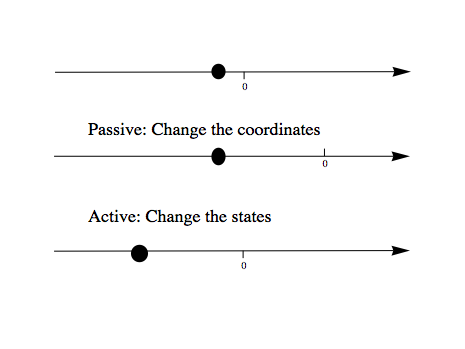
\includegraphics{transformations.png}

Here in QM, passive means transform the operator $\hat \Omega$, while active means change the state $\ket{\psi}$. Suppose we have a system $\ket{\psi}$, an operator $\hat \Omega$, a transformation $\hat U$.

Transformation $\hat U \ket{\psi}$ is identical to $\hat U^\dagger \hat \Omega \hat U$ because they give the same observation results. The first one is called active, while the second one is called passive.


\subsubsection{Parity}
\label{QuantumMechanics:id2}

\paragraph{Definition}
\label{QuantumMechanics:definition}\begin{gather}
\begin{split}\hat \Pi \ket{x}= \ket{-x}\end{split}\notag\\\begin{split}\end{split}\notag
\end{gather}

\paragraph{Properties}
\label{QuantumMechanics:properties}\begin{enumerate}
\item {} 
Act on momentum eigenvectors,
\begin{gather}
\begin{split}\hat \Pi \ket{p} = \ket{-p} .\end{split}\notag\\\begin{split}\end{split}\notag
\end{gather}
\end{enumerate}
\begin{itemize}
\item {} 
Physics: Parity changes the coordinate, so the direction of momentum is also changed.

\item {} 
Math:
\begin{gather}
\begin{split}\hat \Pi \ket{p} = \int \hat \Pi \ket{x}\braket{x}{p}\d x= \int \ket{-x}\braket{x}{p}\d x\end{split}\notag\\\begin{split}\end{split}\notag
\end{gather}
Change coordinate from x to -x,
\begin{gather}
\begin{split}\hat \Pi \ket{p} = \int \ket{x}\braket{-x}{p}\d x = \int \ket{x}\braket{x}{-p}\d x  = \ket{-p}\end{split}\notag\\\begin{split}\end{split}\notag
\end{gather}
\end{itemize}
\begin{enumerate}
\setcounter{enumi}{1}
\item {} 
Hermitian,
\begin{gather}
\begin{split}\bra{x}\hat \Pi \ket{x'} = \delta(x+x')
(\bra{x'}\hat \Pi \ket{x})^\dagger = \bra{x}\hat \Pi^\dagger \ket{x'} =\delta(x+x')\end{split}\notag\\\begin{split}\end{split}\notag
\end{gather}
\item {} 
Unitary
\begin{gather}
\begin{split}\bra{x}\hat \Pi^\dagger \hat \Pi \ket{x'}= \braket{-x}{-x'}=\delta(-x+x')=\delta(x-x')=\braket{x}{x'}\end{split}\notag\\\begin{split}\end{split}\notag
\end{gather}
\item {} 
Inverse of parity
\begin{gather}
\begin{split}\hat \Pi \hat \Pi = \hat \Pi \hat \Pi^\dagger = \hat I\end{split}\notag\\\begin{split}\end{split}\notag
\end{gather}
\item {} 
Eigensystem of parity.
\begin{gather}
\begin{split}\hat \Pi \ket{\pi}=\pi\ket{\pi}\end{split}\notag\\\begin{split}\end{split}\notag
\end{gather}
Apply another operator
\begin{gather}
\begin{split}\hat \Pi^2 \ket{\pi} = \pi^2 \ket{\pi}\end{split}\notag\\\begin{split}\end{split}\notag
\end{gather}
So,
* Eigenvalues: 1, -1;
* Eigenvactors: Even function, Odd function

\item {} 
Parity applied to operators
a. Apply to position operator,
\begin{quote}
\begin{gather}
\begin{split}\hat \Pi^\dagger \hat X \hat \Pi = -\hat X\end{split}\notag\\\begin{split}\end{split}\notag
\end{gather}
Proof:
\begin{gather}
\begin{split}\bra{x}\hat \Pi ^\dagger \hat X \hat \Pi \ket{x'} = \bra{-x}\hat X \ket{-x'}= -x'\delta(x-x') = \bra{x}(-\hat X)\ket{x'}\end{split}\notag\\\begin{split}\end{split}\notag
\end{gather}\end{quote}
\begin{enumerate}
\setcounter{enumi}{1}
\item {} 
Apply to momentum operator,
\begin{gather}
\begin{split}\hat \Pi^\dagger \hat p \hat \Pi = -\hat p\end{split}\notag\\\begin{split}\end{split}\notag
\end{gather}
Proof: Similar to the previous one, just change x basis to momentum basis.

\end{enumerate}

\item {} 
Symmetry related to Hamiltonian.
\begin{gather}
\begin{split}\left[ \hat \Pi , \hat H  \right] = 0\end{split}\notag\\\begin{split}\end{split}\notag
\end{gather}
When this happens, parity of Hamiltonian won't change the wave function. Or the wave function should have an specific parity for 1D problem.

\end{enumerate}


\subsection{Classical Limit of QM}
\label{QuantumMechanics:classical-limit-of-qm}

\subsubsection{Ehrenfest's Theorem}
\label{QuantumMechanics:ehrenfest-s-theorem}
Schrödinger equation and its adjoint
\begin{gather}
\begin{split}i\hbar \frac{\d }{\d t} \ket{\psi(t)} = \hat H \ket{\psi(t)}\end{split}\notag\\\begin{split}-i\hbar \frac{\d }{\d t} \bra{\psi(t)} = \bra{\psi(t)} \hat H\end{split}\notag
\end{gather}
For any observable $\hat \Omega$,
\begin{gather}
\begin{split}\begin{eqnarray}
\frac{\d }{\d t}\left<\hat \Omega \right > &=& \left( \frac{\d}{\d t}\bra{\psi(t)}\right)  \hat \Omega \ket{\psi(t)} + \bra{\psi(t)} \dot{\hat \Omega} \ket{\psi(t)} + \bra{\psi(t)} \hat \Omega \left( \frac{\d}{\d t}\ket{\psi(t)}\right)  \\\\
&=& \frac{1}{i\hbar} \left ( - \bra{\psi(t)} \hat H \hat\Omega \ket{\psi(t)} +\bra{\psi(t)} \hat\Omega \hat H \ket{\psi(t)} \right) + \bra{\psi(t)} \dot{\hat \Omega} \ket{\psi(t)} \\\\
&=& \frac{1}{i\hbar} \bra{\psi(t)}\left[\hat\Omega,\hat H\right] \ket{\psi(t)}+\bra{\psi(t)} \dot{\hat \Omega} \ket{\psi(t)}
\end{eqnarray}\end{split}\notag
\end{gather}
This is called Ehrenfest's Theorem.


\paragraph{Simple Example of Ehrenfest's Theorem}
\label{QuantumMechanics:simple-example-of-ehrenfest-s-theorem}
Suppose we have a system with Hamiltonian
\begin{gather}
\begin{split}\hat H = \frac{\hat p^2}{2m} + V(\hat x)\end{split}\notag\\\begin{split}\end{split}\notag
\end{gather}
We need to figure some commutators first.
\begin{gather}
\begin{split}2m \left[ \hat x, \hat H \right] =\left[\hat x, \hat p^2\right] = \hat x \hat p\hat p - \hat p \hat p \hat x = \hat x \hat p \hat p -\hat p \hat x \hat p + \hat p \hat x \hat p - \hat p \hat p \hat x  = \left[\hat x , \hat p\right]\hat p + \hat p \left[ \hat x,\hat p\right]  = 2 i \hbar \hat p\end{split}\notag\\\begin{split}\end{split}\notag
\end{gather}\begin{gather}
\begin{split}\left[\hat p, \hat H\right] = \left[\hat p, V(\hat x) \right] = \left[\hat p, \sum_0^\infty \frac{V^{(n)}}{n!}\hat x^n\right] =\cdots =-i\hbar V'(\hat x)\end{split}\notag\\\begin{split}\end{split}\notag
\end{gather}\begin{enumerate}
\item {} 
Position average
\begin{gather}
\begin{split}\begin{eqnarray}
\frac{\d }{\d t} \left< \hat x \right> &=& \frac{1}{i\hbar} \bra{\psi(t)} \left[ \hat x, \hat H \right]\ket{\psi(t)} \\\\
&=&  \frac{\left< \hat p \right>}{m}
\end{eqnarray}\end{split}\notag\\\begin{split}\end{split}\notag
\end{gather}
We are familiar with this in classical mechanics.

\item {} 
Momentum average
\begin{gather}
\begin{split}\begin{eqnarray}
\frac{\d}{\d t} \left<\hat p\right> &=& \frac{1}{i\hbar} \bra{\psi(t)} \left[\hat p, \hat H\right] \ket{\psi(t)} \\\\
&=& \frac{1}{i\hbar} \bra{\psi(t)}  (-i\hbar V'(\hat x))  \ket{\psi(t)}  \\\\
&=& -\left< V'(\hat x) \right>
\end{eqnarray}\end{split}\notag\\\begin{split}\end{split}\notag
\end{gather}
In classical mechanics, the derivative of potential is force. And the result is just like Newton's 2n Law except the right hand side is not exactly like a force which should be $-\frac{\d}{\d x} \left< V(\hat x) \right>$.

\end{enumerate}


\paragraph{What does $-\left< V'(\hat x)\right>$ mean}
\label{QuantumMechanics:what-does-mean}
Suppose the potential area is fairly small and distributed around some coordinate $x_0=\left< \hat x \right>$, we can do Taylor expansion around $x_0$.
\begin{gather}
\begin{split}\begin{eqnarray}
< V(\hat x)> &=& V(x_0)   +  V'(x_0) < (x - x_0)> + V''(x_0)<(x-x_0)^2> /2 + \cdots \\\\
&=& V(x_0) + 0 + V''(x_0) (\Delta x)^2 + \cdots
\end{eqnarray}\end{split}\notag\\\begin{split}\end{split}\notag
\end{gather}
If the uncertainty is small enough, every term except the first one becomes small. So to the lowest order, average of potential is approximately the potential at $x_0$.

Similarly, the average of first derivative of potential $<V'(\hat x)>$ is approximately $V'(x_0)$.

These gives us a hint for the previous result we got for the time evolution of average momentum. The result reduces to classical mechanics one as long as we keep the lowest order of Taylor expansion. Those higher order terms show the quantum effect.


\subsubsection{Picture}
\label{QuantumMechanics:picture}
We can see deeper into Ehrenfest's Theorem through Heisenberg Picture of quantum mechanics.


\paragraph{Schrödinger \& Heisenberg Pictures}
\label{QuantumMechanics:schrodinger-heisenberg-pictures}
Pictures are the ways we look at the evolution of systems.


\subparagraph{Schrödinger Picture}
\label{QuantumMechanics:schrodinger-picture}
In Schrödinger picture the states are evolving with time.
\begin{gather}
\begin{split}i\hbar \frac{\d}{\d t} \ket{\psi} _ S = \hat H \ket{\psi} _ S\end{split}\notag\\\begin{split}\end{split}\notag
\end{gather}
And for time independent Hamiltonian,
\begin{gather}
\begin{split}\ket{\psi}_S = U^\dagger \ket{\psi _ 0} _ S\end{split}\notag\\\begin{split}\end{split}\notag
\end{gather}

\subparagraph{Heisenberg Picture}
\label{QuantumMechanics:heisenberg-picture}
In Heisenberg Picture, the states do not change with time.
\begin{gather}
\begin{split}\ket{\psi} _ H = \ket{\psi_0} _ H ,\end{split}\notag\\\begin{split}\end{split}\notag
\end{gather}
and of course the initial is the same with Schrödinger Picture,
\begin{gather}
\begin{split}\ket{\psi_0} _ H = \ket{\psi _ 0} _ S .\end{split}\notag\\\begin{split}\end{split}\notag
\end{gather}
How do we relate to Heisenberg Picture to Schrödinger Picture? Through investigation of observables. We should have the same observation results in both Pictures.
\begin{gather}
\begin{split}  \begin{eqnarray}
  {} _ H \bra{\psi} \hat \Omega _ H \ket{\psi} _ H &=& {} _ S \bra{\psi} \hat \Omega _ S \ket{\psi} _ S \\\\
  {} _ H \bra{\psi} \hat \Omega _ H \ket{\psi} _ H &=& {} _ S \bra{\psi _ 0} \hat U^\dagger \hat \Omega _ S  \hat U \ket{\psi _ 0} _ S \\\\
  \hat \Omega _ H &=& \hat U^\dagger \hat \Omega _ S \hat U
  \end{eqnarray}\end{split}\notag\\\begin{split}So the operators change with time in Heisenberg Picture.\end{split}\notag
\end{gather}

\paragraph{Ehrenfest's Theorem in Heisenberg Picture}
\label{QuantumMechanics:ehrenfest-s-theorem-in-heisenberg-picture}\begin{gather}
\begin{split}\frac{\d }{\d t} \hat \Omega _ H = \frac{1}{i\hbar } \left[ \hat \Omega _ H, \hat H \right] + \hat U ^ \dagger \frac{\partial }{\partial t} \Omega _ H \hat U\end{split}\notag\\\begin{split}\end{split}\notag
\end{gather}
This can be easily proved by throwing every definition need in to it. We also need the following equations.
\begin{gather}
\begin{split}\frac{\d }{\d t} \hat U = \frac{\d }{\d t} e^{-i\hat H t /\hbar} = \frac{\hat H}{i\hbar} \hat U\end{split}\notag\\\begin{split}\end{split}\notag
\end{gather}
And REMEMBER that propagator commute with time independent Hamiltonian, so
\begin{gather}
\begin{split}\hat H = \hat U^\dagger \hat U \hat H = \hat U^ \dagger \hat U \hat U \equiv \hat H _ H\end{split}\notag\\\begin{split}\end{split}\notag
\end{gather}
So this Ehrenfest's Theorem can also be written as
\begin{gather}
\begin{split}\frac{\d }{\d t} \hat \Omega _ H = \frac{1}{i\hbar } \left[ \hat \Omega _ H, \hat H _ H \right] + \hat U ^ \dagger \frac{\partial }{\partial t} \Omega _ H \hat U\end{split}\notag\\\begin{split}\end{split}\notag
\end{gather}
We can \textbf{define}
\begin{gather}
\begin{split}\frac{\partial}{\partial t}\hat  \Omega _ H \equiv \hat U^\dagger  \frac{\partial }{\partial t}\hat  \Omega _ S \hat U  ,\end{split}\notag\\\begin{split}\end{split}\notag
\end{gather}
which is the time derivative of operator in Heisenberg Picture.

\textbf{Reminder: The time derivative of an observable (average) depends not only the time derivative of itself, but also the commutator of the observable and Hamiltonian.}


\subparagraph{Example of Ehrenfest's Theorem in Heisenberg Picture}
\label{QuantumMechanics:example-of-ehrenfest-s-theorem-in-heisenberg-picture}
We will show why it is better to work in Heisenberg Picture to show the meanings of Ehrenfest's Theorem.

Suppose we have a Hamiltonian in Heisenberg Picture,
\begin{gather}
\begin{split}\hat H_H = \frac{\hat p _ H^2 }{2m} + V(\hat x _ H) .\end{split}\notag\\\begin{split}\end{split}\notag
\end{gather}
Time derivative of position operator
\begin{gather}
\begin{split}\frac{\d}{\d t} \hat x _ H = \frac{1}{i\hbar} \left[\hat x _ H, \hat H _ H \right ] = \frac{\hat p _ H}{m}\end{split}\notag\\\begin{split}\end{split}\notag
\end{gather}
Time derivative of momentum operator
\begin{gather}
\begin{split}\frac{\d}{\d t} \hat p_H = \frac{1}{i\hbar } \left[ \hat p _ H, \hat H \right] = - V'(\hat x_H)\end{split}\notag\\\begin{split}\end{split}\notag
\end{gather}
So the operator in Heisenberg Picture just have a sense of the physical quantities in classical mechanics. That's why we like it.


\subsubsection{Conservation}
\label{QuantumMechanics:conservation}
We say a observable is conserved if the corresponding operator commutes with Hamiltonian,
\begin{gather}
\begin{split}\left[ \hat \Omega, \hat H \right]=0\end{split}\notag\\\begin{split}\end{split}\notag
\end{gather}
1. Energy
Hamiltonian always commutes with itself.
\begin{gather}
\begin{split}\frac{\d}{\d t} \left<\epsilon \right> = \bra{\psi} \left( \frac{\partial }{\partial t} \hat H \right) \ket{\psi}\end{split}\notag\\\begin{split}\end{split}\notag
\end{gather}
If Hamiltonian is time independent, then energy is conserved. (If Hamiltonian is tide dependent, energy is not conserved. This is kind of obvious in classical mechanics.)


\paragraph{What is the nature of time dependence}
\label{QuantumMechanics:what-is-the-nature-of-time-dependence}
We can see this by looking at a simple example.

Assume we have a system with energy eigenstates $\ket{\epsilon _ n}$, and initially,
\begin{gather}
\begin{split}\ket{\psi _ 0} = \sum_n C _ n \ket{\epsilon _ n} .\end{split}\notag\\\begin{split}\end{split}\notag
\end{gather}
So
\begin{gather}
\begin{split}\ket{\psi(t)} = \sum _ n C _ n e^{-i\epsilon _ n t/\hbar} \ket{\epsilon _ n} .\end{split}\notag\\\begin{split}\end{split}\notag
\end{gather}
We can calculate the expectation value of some operator $\hat \Omega$,
\begin{gather}
\begin{split}\left< \omega (t) \right> =  \sum _ {n,m} \left( C _ n^ * e^{i\epsilon _ n t/\hbar } \bra{\epsilon _ n} \right)  \hat \Omega \left( C _ m e^{-i \epsilon _ m t/\hbar} \ket{\epsilon _ m} \right) = \sum _ {n,m} C _ n ^* C _ m e^{-i(\epsilon _ m - \epsilon _ n) t/\hbar} \bra{\epsilon _ n} \hat \Omega \ket{\epsilon _ m}\end{split}\notag\\\begin{split}\end{split}\notag
\end{gather}
If $\ket{\epsilon _ n}$ are also the eigenvectors of $\hat \Omega$, then
\begin{gather}
\begin{split}\bra{\epsilon _ n} \hat \Omega \ket{\epsilon _ m} = \omega _ m \delta _ {n,m}\end{split}\notag\\\begin{split}\end{split}\notag
\end{gather}
And the expectation value
\begin{gather}
\begin{split}\left<  \omega (t) \right> = \sum _ {n} C _ n^* C _ n \omega _ n\end{split}\notag\\\begin{split}\end{split}\notag
\end{gather}
\textbf{The important thing is that the time dependence of this expectation value actually arise from this term}
\begin{gather}
\begin{split}e^{-i(\epsilon _ m - \epsilon _ n)t/\hbar} .\end{split}\notag\\\begin{split}\end{split}\notag
\end{gather}
As it is so important, we call
\begin{gather}
\begin{split}(\epsilon _ m - \epsilon _ n)/\hbar\end{split}\notag\\\begin{split}\end{split}\notag
\end{gather}
\textbf{Bohr frequency}.


\subsection{Harmonic Oscillators}
\label{QuantumMechanics:harmonic-oscillators}

\subsubsection{Why Harmonic Oscillators}
\label{QuantumMechanics:why-harmonic-oscillators}
Many systems can reduce to it. Use Taylor expansion for the potential and redefine parameters we will find harmonic oscillators in the potential.

Hamiltonian for 1D is
\begin{gather}
\begin{split}\hat H = \frac{\hat p^2}{2m} + \frac{1}{2} k \hat x^2\end{split}\notag\\\begin{split}\end{split}\notag
\end{gather}

\subsubsection{Standard Solution}
\label{QuantumMechanics:standard-solution}
We can use polynomial expansion for part of the solution.


\paragraph{Dimension Schrodinger Equation}
\label{QuantumMechanics:dimension-schrodinger-equation}
First step is always finding out the characteristic length scale and characteristic energy scale. Assume we have an characteristic length $\eta$ and characteristic energy scale $\epsilon_0$. Through uncertainty principle we know only for dimensional analysis
\begin{gather}
\begin{split}\left[\hat p\right]=\frac{\hbar}{\eta}\end{split}\notag\\\begin{split}\end{split}\notag
\end{gather}
Kinetic energy and potential energy have the same dimension
\begin{gather}
\begin{split}\frac{\hbar^2}{\eta^2 m}=k \eta^2 ,\end{split}\notag\\\begin{split}\end{split}\notag
\end{gather}
so we have
\begin{gather}
\begin{split}\eta = \sqrt{\frac{\hbar}{m\omega}}\end{split}\notag\\\begin{split}\end{split}\notag
\end{gather}
with $\omega^2=k/m$. A dimensional analysis shows that $\epsilon_0=\hbar\omega$.

Now we can define dimensionless variables,
\begin{gather}
\begin{split}z=x/\eta, e=\epsilon/\epsilon_0\end{split}\notag\\\begin{split}\end{split}\notag
\end{gather}
The time independent Schrodinger equation in position basis is
\begin{gather}
\begin{split}-\hbar^2 \frac{\mathrm d^2}{\mathrm dx^2}\psi'' /m + k x^2 = 2\epsilon \psi .\end{split}\notag\\\begin{split}\end{split}\notag
\end{gather}
Using those characteristic scales, we can rewrite this equation into a dimensionless one, which is
\begin{gather}
\begin{split}\psi''+(2e-z^2)\psi = 0\end{split}\notag\\\begin{split}\end{split}\notag
\end{gather}
in which $\psi'=\frac{\mathrm d}{\mathrm dz}\psi$.


\paragraph{Take Limits}
\label{QuantumMechanics:take-limits}
We need to look at the behavior of the solutions before we can guess a proper general solution.

$z\rightarrow \infty$, we have $\psi''-z^2\psi=0$. Solution to this equation is $\psi(z)~ e^{-z^2/2}$.

The solution of the the equation should be in the form
\begin{gather}
\begin{split}\psi(z) = u(z) e^{-z^2/2}  .\end{split}\notag\\\begin{split}\end{split}\notag
\end{gather}
Insert this to time independent Schrodinger equation, we can get the equation of $u(z)$.
\begin{gather}
\begin{split}u'' - 2 z u' +(2e-1) u = 0\end{split}\notag\\\begin{split}\end{split}\notag
\end{gather}

\paragraph{Polynomial Method}
\label{QuantumMechanics:polynomial-method}
The simplest form of $u(z)$ is polynomial,
\begin{gather}
\begin{split}u(z) = \sum _ {n=0}^{\infty} u _ n z^n  .\end{split}\notag\\\begin{split}\end{split}\notag
\end{gather}
Put this back to equation of u, we can get the recursion relation,
\begin{gather}
\begin{split}(n + 2)(n+1) u _ {n+2} = \left[ 2n - (2e - 1) \right] u _ n   .\end{split}\notag\\\begin{split}\end{split}\notag
\end{gather}
If $u_0$ and $u_1$ are given, we can get the whole polynomial.

Notice that we have definite parity here. So $u _ 1$ branch vanish because they are even.

$u_0$ is set by the normalization condition.


\paragraph{Terminate The Series}
\label{QuantumMechanics:terminate-the-series}
The series blow up if it doesn't terminate. So we need to terminate the series using the following relation,
\begin{gather}
\begin{split}2e - 1 = 2n .\end{split}\notag\\\begin{split}\end{split}\notag
\end{gather}
Then we have the energy levels, which is $e=n+1/2$.


\paragraph{Complete Series}
\label{QuantumMechanics:complete-series}
By picking proper normalization factor, we can write down the energy levels and corresponding wave functions. In fact, this polynomial can be found in mathematical phyisics books.
\begin{gather}
\begin{split}H _ {n+1} = 2 z H _n -n H _ {n-1}\end{split}\notag\\\begin{split}\end{split}\notag
\end{gather}

\subsubsection{Tricky Solution}
\label{QuantumMechanics:tricky-solution}
Find out the characteristic length and energy
\begin{gather}
\begin{split}\eta = \sqrt{\frac{\hbar }{m\omega }} \\\\
\epsilon = \hbar \omega \\\\
\omega = \sqrt{\frac{k}{m}}\end{split}\notag\\\begin{split}\end{split}\notag
\end{gather}
One way to get the intrinsic length without writing down the dimensions of each quantity is to use the following relation
\begin{gather}
\begin{split}\left[ E \right] = \left[ m \omega^2 \hat x^2 \right] \\\\
\hbar \omega = m \omega^2 \eta^2 \\\
\eta = \sqrt{ \frac{\hbar}{m\omega} }\end{split}\notag\\\begin{split}\end{split}\notag
\end{gather}
Or if we are given the Hamiltonian in terms of $k$,
\begin{gather}
\begin{split}\left[ \frac{\hat p^2}{2m} \right] = \left[ k \hat x^2 \right] \\\\
\frac{\hbar^2 / \eta^2 }{m} = k\eta^2 \\\\
\eta = \sqrt{\hbar}{ \sqrt{m k} } = \sqrt{ \hbar }{ m \omega }\end{split}\notag\\\begin{split}\end{split}\notag
\end{gather}
Rewrite the Hamiltonian
\begin{gather}
\begin{split}\begin{eqnarray}
\hat H &=& \frac{1}{2m} \left[ \left(\frac{\hat p}{\hbar/\eta}\right)^2 \left(\frac{\hbar}{\eta}\right)^2 + \frac{1}{2} m \omega^2 \left( \frac{\hat x}{\eta} \right)^2 \right] \\\\
&=& \frac 1 2 \hbar \omega \left[ \left(\frac{\hat p}{\hbar/\eta}\right)^2 + \left(\frac{\hat x}{\eta}\right)^2 \right]    \\\\
&=& \frac 1 2 \hbar \omega \left( \frac{\hat x}{\eta} - i \frac{\hat p}{\hbar/\eta}   \right) \left( \frac{\hat x}{\eta} + i\frac{\hat p}{\hbar/\eta}  \right)  - \frac{i}{\hbar} \left[\hat x, \hat p\right]    \\\\
&=& \frac 1 2 \hbar \omega (\sqrt 2 \hat a^\dagger \sqrt 2 \hat a + 1) \\\\
&=& \hbar \omega \left( \hat a^\dagger \hat a + \frac 1 2\right)
\end{eqnarray}\end{split}\notag\\\begin{split}\end{split}\notag
\end{gather}
Now we can define $\hat a^\dagger \hat a = \hat N$, which is just like an operator for (energy) quanta numbers.

An impoertan relation is
\begin{gather}
\begin{split}\left[\hat a, \hat a^\dagger\right] = 1 \\\\
\left[\hat a, \hat N\right] = \hat a\end{split}\notag\\\begin{split}\end{split}\notag
\end{gather}
The eigen equation for this weird energy quanta number operator is
\begin{gather}
\begin{split}\hat N \ket{n} = n \ket{n}\end{split}\notag\\\begin{split}\end{split}\notag
\end{gather}
To find out the eigen state of $\hat a$ and $\hat a^\dagger$, we try this,
\begin{gather}
\begin{split}\hat N (\hat a \ket{n}) = (n-1) (\hat a \ket{n})  \\\\
\hat N (\hat a^\dagger \ket{n}) = (n+1) (\hat a^\dagger \ket{n})\end{split}\notag\\\begin{split}\end{split}\notag
\end{gather}
This means $\hat a \ket{n}$ and $\hat a^\dagger \ket{n}$ are also eigen states of $hat N$.

The next step is very crucial. Since $\hat a \ket{n}$ and $\hat a^\dagger \ket{n}$ are eigen states of $hat N$, we know that
\begin{gather}
\begin{split}\hat a \ket{n} = C1 \ket{n} \\\\
\hat a^\dagger \ket{n} = C2 \ket{n}\end{split}\notag\\\begin{split}\end{split}\notag
\end{gather}
Then our next step is to find out what are $C1$ and $C2$ exactly.

They way of finding them is to use invariant quantities, such as the inner product. Here we use average of $\hat N$ operator.
\begin{gather}
\begin{split}\hat a \ket{n} = \sqrt n \ket{n-1}  \\\\
\hat a^\dagger \ket{n} = \sqrt{n+1} \ket{n+1}\end{split}\notag\\\begin{split}\end{split}\notag
\end{gather}
Final step is to constrain on $n$, which should be integrals. This is true because we need a cut off for the eigen equation of $\hat N$, whose avarage is n and it should be non negative.
\begin{gather}
\begin{split}\bra{n}\hat N \ket{n} \ge 0\end{split}\notag\\\begin{split}\end{split}\notag
\end{gather}
leads to $n\ge 0$. To get this proper cut off, $n$ should be integer because if it's not, according to
\begin{gather}
\begin{split}\hat a \ket{n} = \sqrt n \ket{n-1}\end{split}\notag\\\begin{split}\end{split}\notag
\end{gather}
n can go to negative numbers. If n is positive integer,
\begin{gather}
\begin{split}\hat a \ket{1} = \ket{0}  \\\\
\hat a \ket{0} = 0 \ket{0}\end{split}\notag\\\begin{split}\end{split}\notag
\end{gather}
show an cut off at 0.

We can even find out the wave functions of these $\ket{n}$ by finding the ground state first and apply $\hat a^\dagger$ to the ground state.

Ground state in ${\ket{x}}$ basis can be found by solving the differential equation,
\begin{gather}
\begin{split}\bra{x} \hat a \ket{0} = 0\end{split}\notag\\\begin{split}\end{split}\notag
\end{gather}\begin{quote}

Very important:
\begin{itemize}
\item {} 
The Hermitian conjugate of $\hat a \ket{n}$ is $\bra{n} \hat a^\dagger$.

\item {} 
Hermitian conjugate of $\hat a \hat a^\dagger$ is $\hat a \hat a^dagger$. This can be a trap. Hermitian conjugate is the complex conjugate AND TRANSPOSE!

\end{itemize}
\end{quote}


\subsubsection{Semiclassical}
\label{QuantumMechanics:semiclassical}

\paragraph{Classical}
\label{QuantumMechanics:classical}
In phase space, the trajectory of phase space points ( \{$x/\eta$ and $p/(\hbar/\eta)$\} ) is on a circle of radius $x_{max}/\eta$.


\paragraph{Quantum semiclassical}
\label{QuantumMechanics:quantum-semiclassical}
Key points:
\begin{enumerate}
\item {} 
What is the trajectory of $\left<\hat x/\eta\right>$ and $\left<\hat p/(\hbar/\eta)\right>$

\item {} 
Can we make the trajectory just like the classical case by choosing some special conditions?

\item {} 
What do these special cases mean?

\end{enumerate}
\begin{itemize}
\item {} 
Expectation value of creation and annihilation operators

\end{itemize}

Apply Ehrenfest theorem to annihilation operator,
\begin{gather}
\begin{split}i\hbar \frac{\mathrm d}{\mathrm d t} \avg{\hat a(t)} = \bra{\psi} \left[ \hat a(t), \hat H \right] \ket{\psi} = \hbar \omega \avg{\hat a(t)}\end{split}\notag\\\begin{split}\end{split}\notag
\end{gather}
Excellent. Now we can solve out $\avg{\hat a(t)}$, which is
\begin{gather}
\begin{split}\avg{\hat a(t)} = \alpha_0 \exp(-i\omega t)\end{split}\notag\\\begin{split}\end{split}\notag
\end{gather}
Take the hermitian conjugate,
\begin{gather}
\begin{split}\avg{\hat a^\dagger (t)} = \alpha_0^* \exp(i\omega t)\end{split}\notag\\\begin{split}\end{split}\notag
\end{gather}\begin{itemize}
\item {} 
Expectation value of position and momentum

\end{itemize}

With these two operators, we can find out the average of $\hat x$ and $\hat p$ because
\begin{gather}
\begin{split}\hat x = \eta \frac{1}{\sqrt 2} \left( \hat a^\dagger + \hat a\right)\\\\
\hat p = \frac{\hbar}{\eta} i \frac{1}{\sqrt 2} \left(\hat a^\dagger - \hat a \right) ,\end{split}\notag\\\begin{split}\end{split}\notag
\end{gather}
we have
\begin{gather}
\begin{split}\avg{\hat x(t)} = \eta \frac{1}{\sqrt 2} \left( \avg{\hat a^\dagger (t)} + \avg{\hat a(t)} \right) \\\\
\avg{\hat p(t)} = \frac{\hbar}{\eta} i \frac{1}{\sqrt {2} } \left( \avg{\hat a^\dagger (t) - \avg{\hat a(t)}} \right)\end{split}\notag\\\begin{split}\end{split}\notag
\end{gather}
We can have a look at these two averages,
\begin{gather}
\begin{split}\frac{\avg{\hat x(t)} }{\eta} = \frac{1}{\sqrt{2} } \left[ (\alpha_0 + \alpha_0^*)\cos(\omega t) + i (\alpha_0^* - \alpha_0 ) \sin(\omega t) \right] \\\\
\frac{\avg{\hat p(t)}}{\hbar/\eta} = \frac{1}{\sqrt{2}} \left[ (\alpha_0 + \alpha_0^*) \sin(\omega t) + i( \alpha_0 - \alpha_0^*)\cos(\omega t) \right]\end{split}\notag\\\begin{split}\end{split}\notag
\end{gather}
It is obvious that the average reduces to classical case if $\alpha_0 = \alpha_0^*$. \textbf{But this is too strong for a semiclassical limit.}
\begin{itemize}
\item {} 
Coherent state

\end{itemize}

\textbf{Coherent state is the eigenstate of creation operator. Its wave package has the smallest spread allowed by quantum mechanics.}

\textbf{The most special part about coherent state is that the system stays on coherent state if it start with coherent state.}
\begin{gather}
\begin{split}\hat a \ket{\alpha(t)} = \alpha(t) \ket{\alpha(t)}\end{split}\notag\\\begin{split}\end{split}\notag
\end{gather}
Take the hermitian conjugate,
\begin{gather}
\begin{split}\bra{\alpha(t)} \hat a^\dagger  = \bra{\alpha(t)}\alpha(t)^*\end{split}\notag\\\begin{split}\end{split}\notag
\end{gather}
At $t=0$, we have
\begin{gather}
\begin{split}\bra{\psi(0)} N \ket{\psi(0)} = \vert \alpha_0 \vert ^2\end{split}\notag\\\begin{split}\end{split}\notag
\end{gather}
That is to say, energy should be
\begin{gather}
\begin{split}\bra{\psi(0)} \hat H \ket{\psi(0)} = \hbar \omega \left( \vert \alpha_0 \vert^2 + \frac{1}{2} \right)\end{split}\notag\\\begin{split}\end{split}\notag
\end{gather}
Initially, we also have
\begin{gather}
\begin{split}\bra{\psi(0)} (\hat a - \alpha_0)^\dagger (\hat a-\alpha_0) \ket{\psi(0)} = 0\end{split}\notag\\\begin{split}\end{split}\notag
\end{gather}
This means
\begin{gather}
\begin{split}\hat a \ket{\psi(0)} = \alpha_0 \ket{\psi(0)}\end{split}\notag\\\begin{split}\end{split}\notag
\end{gather}\begin{itemize}
\item {} 
Coherent state expanded using energy eigenstates

\end{itemize}

(This result)

(To Be Finished...)


\section{Quantum Mechanics 2}
\label{QuantumMechanics2:quantum-mechanics-2}\label{QuantumMechanics2::doc}

\subsection{Tensor Product Space}
\label{QuantumMechanics2:tensor-product-space}
This part has been moved to {\hyperref[math:tensorproductspace]{\emph{Tensor Product Space}}}


\subsection{Density Matrix}
\label{QuantumMechanics2:density-matrix}

\subsection{Angular Momentum}
\label{QuantumMechanics2:angular-momentum}\begin{gather}
\begin{split}\newcommand{\ud}[1]{{#1^{\dagger}}}
\newcommand{\bra}[1]{\left\langle #1\right|}
\newcommand{\ket}[1]{\left| #1\right\rangle}
\newcommand\Tr{\mathrm{Tr}}
\newcommand{\braket}[2]{\langle #1 \mid #2 \rangle}
\newcommand\d{\mathrm{d}}
\newcommand\I{\mathbb{I}}
\newcommand{\avg}[1]{\left< #1 \right>}\end{split}\notag\\\begin{split}\end{split}\notag
\end{gather}

\subsubsection{Angular Momentum}
\label{QuantumMechanics2:id1}
For an new operator, we would like to know
\begin{enumerate}
\item {} 
Commutation relation: with their own components, with other operators;

\item {} 
Eigenvalues and their properties;

\item {} 
Eigenstates and their properties;

\item {} 
Expectation and classical limit.

\end{enumerate}


\paragraph{Definition of Angular Momentum}
\label{QuantumMechanics2:definition-of-angular-momentum}
In classical mechanics, angular momentum is defined as
\begin{gather}
\begin{split}\vec L = \vec X \times \vec P .\end{split}\notag\\\begin{split}\end{split}\notag
\end{gather}
One way of defining operator is to change position and momentum into operators and check if the operator is working properly in QM. So we just define
\begin{gather}
\begin{split}\hat {\vec L} = \hat {\vec X}\times \hat{\vec P}.\end{split}\notag\\\begin{split}\end{split}\notag
\end{gather}
It is Hermitian. So it can be an operator. We also find
\begin{gather}
\begin{split}\hat{\vec L}\times \hat{\vec L} = i \hbar \hat{\vec L}\end{split}\notag\\\begin{split}\end{split}\notag
\end{gather}\begin{gather}
\begin{split}\left[\hat L_i,\hat L_j\right] = \sum_k i\epsilon_{ijk}\hat L_k    .\end{split}\notag\\\begin{split}\end{split}\notag
\end{gather}
\textbf{More generally, we can define angular momentum as}
\begin{gather}
\begin{split}\left[\hat J_i, \hat J_j\right] = i\hbar \sum_k \epsilon_{ijk} \hat J_k\end{split}\notag\\\begin{split}\end{split}\notag
\end{gather}
We can prove that
\begin{gather}
\begin{split}\left[ \hat J^2,\hat J_z \right] = 0.\end{split}\notag\\\begin{split}\end{split}\notag
\end{gather}
So they can have the same eigenstates
\begin{gather}
\begin{split}\hat J_z \ket{\lambda m} = m\hbar \ket{\lambda m}\end{split}\notag\\\begin{split}\end{split}\notag
\end{gather}\begin{gather}
\begin{split}\hat J^2 \ket{\lambda m} = \lambda^2 \hbar^2 \ket{\lambda m}\end{split}\notag\\\begin{split}\end{split}\notag
\end{gather}
To find the constraints on these eigenvalues, we can use positive definite condition of certain inner porducts, such as,
\begin{gather}
\begin{split}\bra{\psi} \hat J_+ \hat J_- \ket{\psi} \geq 0\end{split}\notag\\\begin{split}\end{split}\notag
\end{gather}\begin{gather}
\begin{split}\bra{\psi} \hat J_- \hat J_+ \ket{\psi} \geq 0\end{split}\notag\\\begin{split}\end{split}\notag
\end{gather}
where
\begin{gather}
\begin{split}\hat J_{\pm} = \hat J_x \pm i \hat J_y\end{split}\notag\\\begin{split}\end{split}\notag
\end{gather}
and we have
\begin{gather}
\begin{split}\left[\hat J_+, \hat J_-\right] = 2 \hbar \hat J_z\end{split}\notag\\\begin{split}\end{split}\notag
\end{gather}\begin{gather}
\begin{split}\left[\hat J_z, \hat J_{\pm} \right] = \pm \hbar \hat J_{\pm}.\end{split}\notag\\\begin{split}\end{split}\notag
\end{gather}
It's easy to find out that
\begin{gather}
\begin{split}\hat J_z (\hat J_{\pm}\ket{\lambda m}) = (m\pm 1) \hbar (\hat J_{\pm} \ket{\lambda m})\end{split}\notag\\\begin{split}\end{split}\notag
\end{gather}
i.e., $\hat J_{\pm}\ket{\lambda m}$ is eigenstate of $\hat J_z$.

Follow the plan of finding out the bounds through these positive inner products, we can prove that
\begin{gather}
\begin{split}\hat J^2\ket{jm} = j(j+1)\hbar^2 \ket{jm}\end{split}\notag\\\begin{split}\end{split}\notag
\end{gather}\begin{gather}
\begin{split}\hat J_{\pm}\ket{jm} = \sqrt{j(j+1)-m(m\pm 1)} \hbar \ket{j,m\pm 1}\end{split}\notag\\\begin{split}\end{split}\notag
\end{gather}

\paragraph{Eigenstates of Angular Momentum}
\label{QuantumMechanics2:eigenstates-of-angular-momentum}
As we have proposed, the eigenstates of both $\hat J_z$ and $\hat{\vec J}^2$ are $\ket{j,m}$, where $j=0,1,2,\cdots$ and $m=-j,-j+1,\cdots, j-1,j$.

We can also find out the wave function in $\{\ket{\theta,\phi\}$ basis. Before we do that, the definition of this basis should be made clear. This basis spans the surface of a 3D sphere in Euclidean space and satisfies the following orthonormal and complete condition.
\begin{gather}
\begin{split}\int \mathrm d \Omega \braket{\theta',\phi'}{\theta,\phi} = \delta(\cos\theta'-\cos\theta,\phi'-\phi)
\int \mathrm d \Omega \ket{\theta',\phi'}\bra{\theta,\phi} = 1\end{split}\notag\\\begin{split}\end{split}\notag
\end{gather}
Now we have an arbitary state $\ket{\psi}$,
\begin{gather}
\begin{split}\ket{\psi} &= \sum _ {l,m} \psi _ {lm}\ket{l,m} \\
           &= \sum _ {l,m} \int \mathrm d \Omega \ket{\theta',\phi'}\bra{\theta,\phi} \psi _ {lm}\ket{l,m} \\
           &= \sum _ {l,m} \int \mathrm d \Omega \ket{\theta',\phi'} (\braket{\theta,\phi}{l,m} ) \psi _ {lm} \\\end{split}\notag\\\begin{split}\end{split}\notag
\end{gather}
Then we define
\begin{gather}
\begin{split}\braket{\theta,\phi}{l,m}=Y_l^m(\theta,\phi)\end{split}\notag\\\begin{split}\end{split}\notag
\end{gather}
which is the spherical harmonic function.

Then
\begin{gather}
\begin{split}\ket{\psi} &= \sum _ {l,m} \psi _ {lm} \int \mathrm d \Omega   Y_l^m(\theta,\phi) \ket{\theta',\phi'}  \\\end{split}\notag\\\begin{split}\end{split}\notag
\end{gather}
So as long as we find out what $\psi _ {lm}$ is, any problem is done.


\section{Quantum Mechanics 3}
\label{QuantumMechanics3:quantum-mechanics-3}\label{QuantumMechanics3::doc}

\subsection{Approximations}
\label{QuantumMechanics3:approximations}\begin{gather}
\begin{split}\newcommand{\ud}[1]{{#1^{\dagger}}}
\newcommand{\bra}[1]{\left\langle #1\right|}
\newcommand{\ket}[1]{\left| #1\right\rangle}
\newcommand\Tr{\mathrm{Tr}}
\newcommand{\braket}[2]{\langle #1 \mid #2 \rangle}
\newcommand\d{\mathrm{d}}
\newcommand\I{\mathbb{I}}
\newcommand{\avg}[1]{\left< #1 \right>}\end{split}\notag\\\begin{split}\end{split}\notag
\end{gather}

\subsubsection{Variational Method}
\label{QuantumMechanics3:variational-method}
The idea comes from that
\begin{gather}
\begin{split}\avg{E} = \frac{\bra{\psi}\hat H\ket{\psi}}{\bracket{\psi}{\psi}} = \frac{\sum_n \left| \bracket{n}{\psi}  \right|^2}{\sum_n \left| \bracket{n}{\psi} \right|^2} \geq E_n\end{split}\notag\\\begin{split}\end{split}\notag
\end{gather}
if $\ket{\psi}$ is composed only with $\ket{i}$ ($i\geq n$).


\subsubsection{WKB Approximation}
\label{QuantumMechanics3:wkb-approximation}

\section{Statistical Physics}
\label{StatisticalPhysics::doc}\label{StatisticalPhysics:statistical-physics}
This part has been moved to \href{http://emptymalei.github.io/StatisticalPhysics/}{here} .


\section{Special Relativity}
\label{SpecialRelativity::doc}\label{SpecialRelativity:special-relativity}

\subsection{Conventions}
\label{SpecialRelativity:conventions}
Metric in special relativity
\begin{gather}
\begin{split}\begin{equation}\eta_{\mu\nu}=\left(\begin{matrix}
     -1 & 0 & 0 & 0\\
     0 & 1 & 0 & 0\\
     0 & 0 & 1 & 0\\
     0 & 0 & 0 & 1\\
\end{matrix}\right)\end{equation}\end{split}\notag
\end{gather}

\subsubsection{Quantities and Operations}
\label{SpecialRelativity:quantities-and-operations}

\paragraph{d'Alembertian}
\label{SpecialRelativity:d-alembertian}
d'Alembert operator, or wave operator, is the Lapace operator in Minkowski space. \footnote{
Actually, there are more general definations for Lapacian, which includes this d'Alembertian of course.
}
\begin{gather}
\begin{split}\Box\equiv \partial _ \mu\partial^\nu = \eta _{\mu\nu}\partial^\mu \partial^\nu\end{split}\notag
\end{gather}
In the usual \{t,x,y,z\} natural orthonormal basis,
\begin{gather}
\begin{split}\begin{eqnarray}
 \Box&=&-\partial_t^2+\partial_x^2+\partial_y^2+\partial_z^2 \\
 &=&-\partial_t^2+\Delta^2 \\
 &=&-\partial_t^2+\nabla
\end{eqnarray}\end{split}\notag\\\begin{split}\end{split}\notag
\end{gather}\begin{description}
\item[{On wiki \footnote{
wiki:D'Alembert\_operator
} , they give some applications to it.}] \leavevmode\begin{itemize}
\item {} 
klein-Gordon equation
$(\Box+m^2)\phi=0$

\item {} 
wave equation for electromagnetic field in vacuum:
For the electromagnetic four-potential \$Box A\textasciicircum{}mu=0\$footnote\{Gauge\}

\item {} 
wave equation for small vibrations
$\Box_c u(t,x)=0\rightarrow u_{tt}-c^2 u_{xx}=0$

\end{itemize}

\end{description}


\subsubsection{Footnotes}
\label{SpecialRelativity:footnotes}

\section{General Relativity}
\label{GeneralRelativity::doc}\label{GeneralRelativity:general-relativity}

\subsection{Description of Space-time Manifold}
\label{GeneralRelativity:description-of-space-time-manifold}
How to describe space-time manifold?
\begin{itemize}
\item {} 
Metric (with a set of local coordinates), connection (Christoffel symbols).

\item {} 
Metric (in the form of tetrads), connection (Ricci rotation coefficients).

\item {} 
1+3 covariantly defined variables.

\end{itemize}


\subsection{Description of Space-time Manifold - Coordinates}
\label{GeneralRelativity:description-of-space-time-manifold-coordinates}

\subsection{Description of Space-time Manifold - Tetrads}
\label{GeneralRelativity:description-of-space-time-manifold-tetrads}

\subsection{Description of Space-time Manifold - 1+3 Covariant Description}
\label{GeneralRelativity:description-of-space-time-manifold-1-3-covariant-description}
Physics in description is easier to understand.


\subsubsection{Definations}
\label{GeneralRelativity:definations}
Definations of some physical quantities and operators are listed below.

Here we have
\begin{enumerate}
\item {} 
\textbf{geometrical variables}: Volume

\item {} 
\textbf{Kinematical variables}: Velocity, Expansion rate, Shear rate

\item {} 
\textbf{Thermaldynanmical variables}: Energy density, Momentum density, Pressure, Equation of state

\end{enumerate}


\paragraph{Volume}
\label{GeneralRelativity:volume}
To calculate volume, the volume element should be defined first in order to integrate. Before that, orientation on manifolds is to be figured out.

On an oriented manifold with metric, the defined volume element (a n-form) should be compatible with the orientation and also determined by the metric. \footnote{
For more information, check out Canbin Liang's book. Volume 1, page 115.
}

Introducing those requirements, a compatible volume element is
\begin{gather}
\begin{split}\begin{equation}
\epsilon_{a_1\cdots a_n} = \pm \sqrt{|g|} (e^1)_{a_1}\wedge \cdots \wedge (e^n)_{a_n}
\end{equation}\end{split}\notag\\\begin{split}\end{split}\notag
\end{gather}
Alternatively, this can be expressed in the way Ellis used in arXiv:gr-qc/9812046v5.
\begin{gather}
\begin{split}\begin{equation}
\eta_{abcd} = \eta_{[abcd]}, \quad \mathrm{with} \eta_{0123} = \sqrt{|\mathrm {det} g_{ab}|}
\end{equation}\end{split}\notag\\\begin{split}\end{split}\notag
\end{gather}
Induced volume element \$hat epsilon\_\{a\_1cdots a\_\{n-1\}\}\$ is defined use the normal vector \$u\textasciicircum{}a\$ of the hypersurface,
\begin{gather}
\begin{split}\begin{equation}
\hat \epsilon_{a_1\cdots a_{n-1}} = u^b \epsilon_{b a_1 \cdots a_{n-1}}
\end{equation}\end{split}\notag\\\begin{split}\end{split}\notag
\end{gather}

\paragraph{4-velocity}
\label{GeneralRelativity:velocity}
4-velocity of observed matter is
\begin{gather}
\begin{split}u^\alpha = \frac{\mathrm d x^\alpha}{\mathrm d \tau}\end{split}\notag\\\begin{split}\end{split}\notag
\end{gather}
with $u^\alpha u_\alpha =-1$, \$tau\$ is the proper time along the worldlines of investaged matter.


\paragraph{Projection Tensors}
\label{GeneralRelativity:projection-tensors}
We can use 4-velocity to project variables to parts that is parallel to \$u\textasciicircum{}alpha\$ and parts that is orthogonal to $u^\alpha$.
\begin{gather}
\begin{split}\begin{eqnarray}
U^a_{\phantom a b} &=& -u^a u_b \\
h_{ab} &=& g_{ab} + u_a u_b, \qquad \text{induced metric from $g_{ab}$}
\end{eqnarray}\end{split}\notag\\\begin{split}\end{split}\notag
\end{gather}
Some properties of the  two projections.
\begin{gather}
\begin{split}\begin{eqnarray}
&& U^a_{\phantom a b} U^b_{\phantom bc} = U^a_{\phantom a c}  ,  U^a_{\phantom a a} = 1  , U_{ab}=g_{ac} U^c_{\phantom cb}  , U_{ab} u^b = - g_{ac} u^c u_b u^b = u_a \\
&& h^a_{\phantom ab} = g^{ac} h_{cb} = \delta^a_{\phantom ab} + u^a u_b = \delta^a_{\phantom ab} - U^a_{\phantom ab} \\
&& h^a_{\phantom a c}h^c_{\phantom c b} = (\delta^a_{\phantom ac} - U^a_{\phantom ac})(\delta^c_{\phantom cb} - U^c_{\phantom cb}) = \delta^a_{\phantom ab} - U^a_{\phantom ab} = h^a_{\phantom ab} \\
&& h^a_{\phantom aa} = 4-1 = 3  ,   h_{ab}u^b = 0
\end{eqnarray}\end{split}\notag\\\begin{split}\end{split}\notag
\end{gather}

\paragraph{Covariant time derivative ($\dot \quad$)}
\label{GeneralRelativity:covariant-time-derivative}
This is the derivative along the fundamental worldlines (projection on the worldlines),
\begin{gather}
\begin{split}\begin{equation}
\dot T^{ab}_{\phantom{ab}cd} = u^e \nabla_e T^{ab}_{\phantom{ab}cd}
\end{equation}\end{split}\notag\\\begin{split}\end{split}\notag
\end{gather}

\paragraph{Fully orthogonally projected covariant derivative ($\tilde \nabla$)}
\label{GeneralRelativity:fully-orthogonally-projected-covariant-derivative}
This derivative is the project orghogonal to the normal vector of the hyperspace or orthogonal to the observer's 4-velocity or along the tagent of the hyperspace.
\begin{gather}
\begin{split}\begin{equation}
     \tilde\nabla_e T^{ab}_{\phantom{ab}cd} = h^a_f h^b_gh^p_ch^q_dh^r_e \nabla_r T^{fg}_{\phantom{fg}pq}
\end{equation}\end{split}\notag\\\begin{split}\end{split}\notag
\end{gather}

\paragraph{Orthogonal projections of vectors}
\label{GeneralRelativity:orthogonal-projections-of-vectors}
Orthogonal projection of vectors
\begin{gather}
\begin{split}\begin{equation}
v^{<a>}      = h^a_{\phantom a b} v^b
\end{equation}\end{split}\notag\\\begin{split}\end{split}\notag
\end{gather}
And the orthogonally projected symmetric trace-free part of tensors
\begin{gather}
\begin{split}\begin{equation}
     T^{<ab>} = [h^{(a}_{\phantom {(a} c} h^{b)}_{\phantom{b)}d} - \frac{1}{3} h^{ab} h_{cd} ] T^{cd}
\end{equation}\end{split}\notag\\\begin{split}\end{split}\notag
\end{gather}

\paragraph{Othogonal projected covariant time derivatives along \$u\textasciicircum{}a\$}
\label{GeneralRelativity:othogonal-projected-covariant-time-derivatives-along-u-a}\begin{gather}
\begin{split}\dot v^{<a>} = h^a_{\phantom a b} \dot v^b\end{split}\notag\\\begin{split}\dot T^{<ab>} = [ h^{(a}_{\phantom{(a}b} h^{b)}_{\phantom{b)} d} - \frac 1 3 h^{ab}h_{cd} ]\dot T^{cd}\end{split}\notag
\end{gather}

\subsubsection{Properties}
\label{GeneralRelativity:properties}\begin{itemize}
\item {} 
Projected time and space derivatives of $U_{ab}$, $h_{ab}$ and $\eta_{abc}$ vanish.

\end{itemize}


\subsection{Fields and Particles}
\label{GeneralRelativity:fields-and-particles}

\subsubsection{Energy-Momentum Tensor for Particles}
\label{GeneralRelativity:energy-momentum-tensor-for-particles}\begin{gather}
\begin{split}\begin{equation}
S_p \equiv -m c \int \int \mathrm d s\mathrm d\tau \sqrt{-\dot x ^\mu g_{\mu\nu} \dot x^\nu} \delta^4(x^\mu - x^\mu (s))    ,
\end{equation}\end{split}\notag\\\begin{split}\end{split}\notag
\end{gather}
in which $x^\mu(s)$ is the trajectory of the particle. Then the energy density \$rho\$ corresponds to $m\delta^4(x^\mu- x^\mu(s))$.

The Largrange density
\begin{gather}
\begin{split}\mathcal L = -\int\mathrm ds mc \sqrt{-\dot x^\mu g_{\mu\nu}\dot x^\nu}\delta^4(x^\mu - x^\mu(s))\end{split}\notag
\end{gather}
Energy-momentum density is $\mathcal T^{\mu\nu} = \sqrt{-g}T^{\mu\nu}$ is
\begin{gather}
\begin{split}\mathcal T^{\mu\nu} = -2 \frac{\partial \mathcal L}{\partial g_{\mu\nu}}\end{split}\notag\\\begin{split}\end{split}\notag
\end{gather}
Finally,
\begin{gather}
\begin{split}\begin{eqnarray}
\mathcal T^{\mu\nu} &=& \int \mathrm ds \frac{mc\dot x^\mu \dot x^\nu}{\sqrt{-\dot x^\mu g_{\mu\nu} \dot x^\nu}} \delta(t-t(s))\delta^3(\vec x - \vec x(t)) \\
&=& m\dot x^\mu \dot x^\nu \frac{\mathrm d s}{\mathrm d t} \delta^3(\vec x - \vec x(s(t)))
\end{eqnarray}\end{split}\notag\\\begin{split}\end{split}\notag
\end{gather}

\subsection{Theorems}
\label{GeneralRelativity:theorems}

\subsubsection{Killing Vector Related}
\label{GeneralRelativity:killing-vector-related}
$\xi^a$ is Killing vector field, $T^a$ is the tangent vector of geodesic line. Then $T^a\nabla_a(T^b\xi_b)=0$, that is $T^b\xi_b$ is a constant on geodesics.


\subsection{Specific Topics}
\label{GeneralRelativity:specific-topics}

\subsubsection{Redshift}
\label{GeneralRelativity:redshift}
In geometrical optics limit, the angular frequency $\omega$ of a photon with a 4-vector $K^a$, measured by a observer with a 4-velocity $Z^a$, is $\omega=-K_aZ^a$.


\subsubsection{Stationary vs Static}
\label{GeneralRelativity:stationary-vs-static}

\paragraph{Stationay}
\label{GeneralRelativity:stationay}
``A stationary spacetime admits a timelike Killing vector field. That a stationary spacetime is one in which you can find a family of observers who observe no changes in the gravitational field (or sources such as matter or electromagnetic fields) over time.''

When we say a field is stationary, we only mean the field is time-independent.


\paragraph{Static}
\label{GeneralRelativity:static}
``A static spacetime is a stationary spacetime in which the timelike Killing vector field has vanishing vorticity, or equivalently (by the Frobenius theorem) is hypersurface orthogonal. A static spacetime is one which admits a slicing into spacelike hypersurfaces which are everywhere orthogonal to the world lines of our `bored observers'''

When we say a field is static, the field is both time-independent and symmetric in a time reversal process.


\section{General Relativity Revisited}
\label{GeneralRelativityAdv:general-relativity-revisited}\label{GeneralRelativityAdv::doc}
This post lists the experiments which are used to test gravity theories
carried out on the earth.

The test of gravity theories can be viewed as test of the fundations of
gravity theories and the the theories themselves, say test of equivalent
principle and general relativity or f(R) gravity theory. Thus we should
break down general relativity theory into several stages. Here, we use
the following table to do so.
\begin{itemize}
\item {} 
\textbf{Physical Fundations: Hyperthesis}:

\end{itemize}

\begin{tabulary}{\linewidth}{|L|L|L|L|L|L|L|}
\hline
\textsf{\relax 
Theory
} & \textsf{\relax 
Mach
} & \textsf{\relax 
WEP
} & \textsf{\relax 
EEP
} & \textsf{\relax 
SEP
} & \textsf{\relax 
GC
} & \textsf{\relax 
Notes
}\\
\hline
GR
 & 
Partial
 & 
Y
 & 
Y
 & 
Y
 & 
Y
 & \\
\hline\end{tabulary}

\begin{itemize}
\item {} 
\textbf{Mathematical Description}:

\end{itemize}

\begin{tabulary}{\linewidth}{|L|L|L|L|L|}
\hline
\textsf{\relax 
Theory
} & \textsf{\relax 
Topoplogy
} & \textsf{\relax 
Manifold
} & \textsf{\relax 
Connection
} & \textsf{\relax 
Metric
}\\
\hline
GR
 &  &  & 
No torsion
 & 
Non-metricity tensor vanishes
\\
\hline\end{tabulary}

\begin{itemize}
\item {} 
\textbf{Theoretical Implifications}:

\end{itemize}

\begin{tabulary}{\linewidth}{|L|L|L|L|L|}
\hline
\textsf{\relax 
Theory
} & \textsf{\relax 
Gravitational Waves
} & \textsf{\relax 
Newtonian Limit
} & \textsf{\relax 
GR Limit
} & \textsf{\relax 
Notes
}\\
\hline
GR
 &  &  &  & \\
\hline\end{tabulary}


Most items in mathematics are the same in different theories.


\subsection{Hyperthesis}
\label{GeneralRelativityAdv:hyperthesis}\begin{itemize}
\item {} 
\textbf{WEP}: weak equivalence principle

\item {} 
\textbf{EEP}: Einstein equivalence principle

\item {} 
\textbf{SEP}: strong equivalence principle

\item {} 
\textbf{GC}, General Covariance

\item {} 
\textbf{Mach Principle}: gravity coupled to matter

\end{itemize}


\subsection{Experiments}
\label{GeneralRelativityAdv:experiments}

\subsubsection{Eotvos Torsion Balance}
\label{GeneralRelativityAdv:eotvos-torsion-balance}

\paragraph{How}
\label{GeneralRelativityAdv:how}\begin{itemize}
\item {} 
Inertial mass $m_I$

\item {} 
Gravitational mass $m_G$

\end{itemize}

In Newtonian system, the acceleration of an object will be \textbackslash{}{[} a \textbackslash{}{]}

In a static and uniform gravitation field, the gravity force is \textbackslash{}{[} G =
- g m\_G r \textbackslash{}{]}

Thus the acceleration in this case should be \textbackslash{}{[} a -r g \textbackslash{}{]}

When $m_G/m_I$ is constant, the falling accerelation are the same
for different objects with same mass. However, if $m_G/m_I$ is not
a constant, say $m_G\ne m_I$, different objects would fall at
different acceleration.

Now if we put two ball with different mass on the Eotvos torsion
balance, the balance would rotate and we can measure it.


\paragraph{Results}
\label{GeneralRelativityAdv:results}
Detection of
$R^k_{0l0}=(1/c^2)\partial^2\Phi/\partial x^k\partial x^l \sim 10^{-32} \text{cm}^{-2}$.


\subsubsection{Hughes-Drevershiy Experiment, etc}
\label{GeneralRelativityAdv:hughes-drevershiy-experiment-etc}
Anisotropy of gravitation/electromagnetism is not proved in our galaxy.


\subsubsection{Radio Signal}
\label{GeneralRelativityAdv:radio-signal}
Similar to Eddington and Dyson's bending light observation, radio
signals serve as a more precise experiment to test Einstein's theory.
And these experiments are against scalar tensor theories because scalar
tensor theories give a smaller bending angle (1.66 second of arc less
than the observations).


\subsection{Summary Table}
\label{GeneralRelativityAdv:summary-table}
Tables constructed according to arXiv:1106.2476v3.

Test of fundamental principles

\begin{tabulary}{\linewidth}{|L|L|L|L|}
\hline
\textsf{\relax } & \textsf{\relax 
Experiment
} & \textsf{\relax 
Results
} & \textsf{\relax 
Note
}\\
\hline
WEP
 & 
Eotvos torsion balance
 & 
$\eta = (0.3 \pm 1.8) \times 10^{-13}$
 & 
More precise in space exp. {[}{[}\textasciicircum{}1{]}a{]} {[}{[}\textasciicircum{}1b{]}{]} {[}{[}\textasciicircum{}1c{]}{]}
\\
 & 
Gravitational redshift of light
 &  & 
{[}{[}\textasciicircum{}2{]}{]}
\\

EEP
 & 
Hughes-Drever Experiment
 &  & \\
\hline\end{tabulary}



\section{Cosmology}
\label{Cosmology/cosmoIndex::doc}\label{Cosmology/cosmoIndex:cosmology}

\subsection{Thermal History of The Universe}
\label{Cosmology/cosmoIndex:thermal-history-of-the-universe}

\subsubsection{Review of Standard Model for Particle Physics}
\label{Cosmology/cosmoIndex:review-of-standard-model-for-particle-physics}\begin{description}
\item[{SM of particle physics}] \leavevmode\begin{enumerate}
\item {} 
describes elementary particles and their interactions.

\item {} 
is well test with experiments.

\end{enumerate}

\end{description}


\paragraph{Degree of Freedom of Elementary Particles}
\label{Cosmology/cosmoIndex:degree-of-freedom-of-elementary-particles}
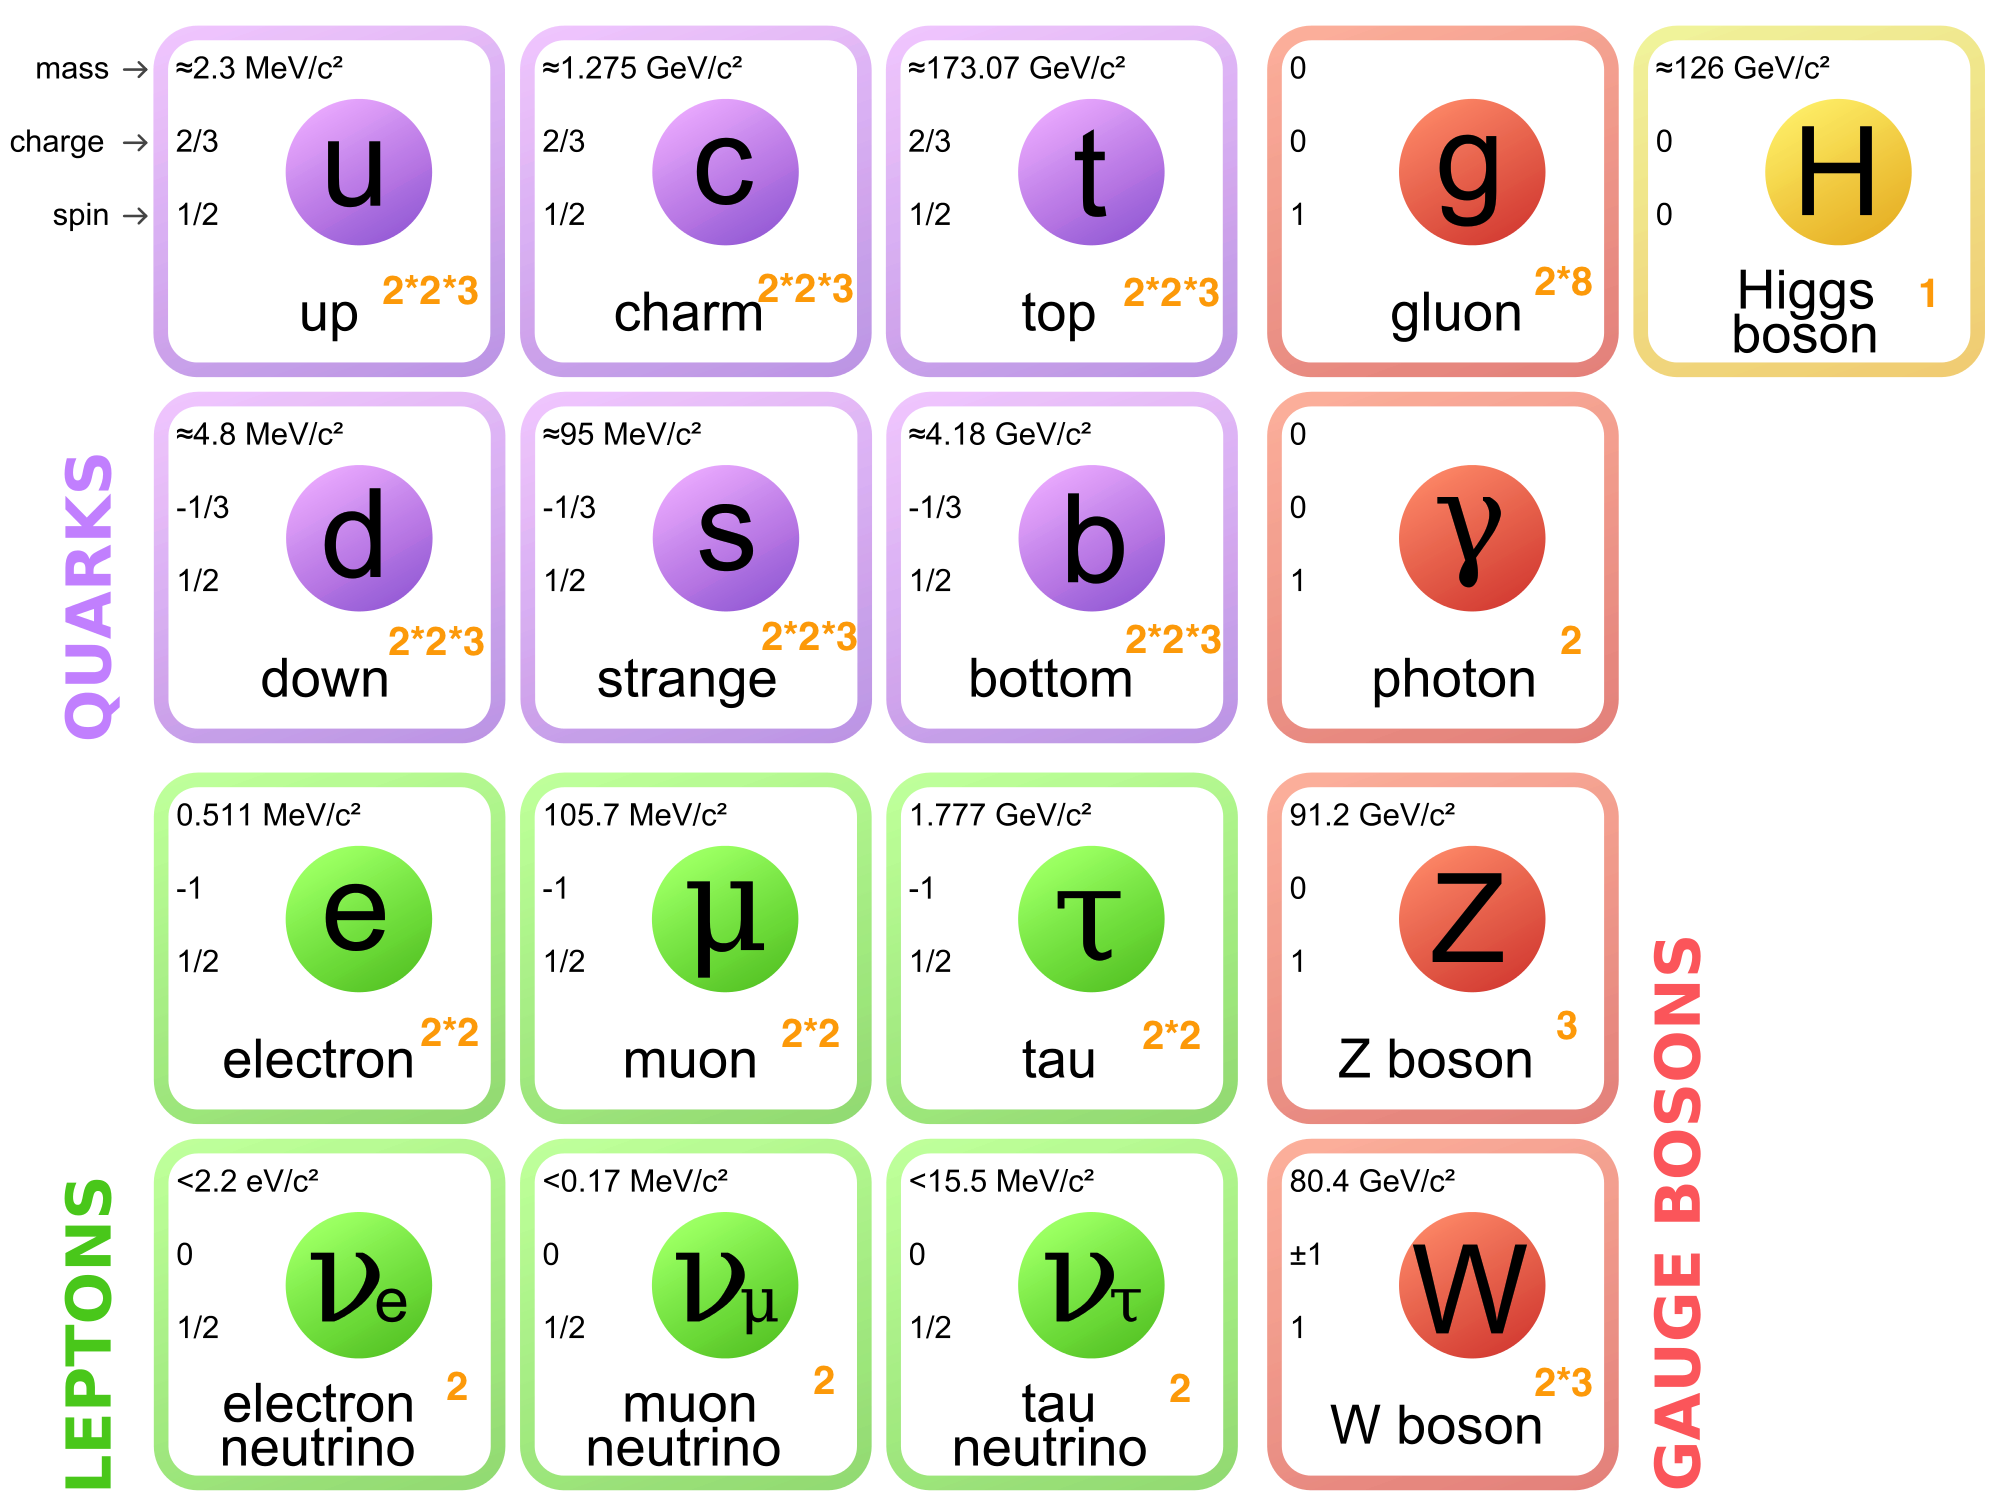
\includegraphics{Standard_Model_of_Elementary_Particles.png}

IMG Source: \href{https://en.wikipedia.org/wiki/File:Standard\_Model\_of\_Elementary\_Particles.svg}{https://en.wikipedia.org/wiki/File:Standard\_Model\_of\_Elementary\_Particles.svg}

The orange numbers at the right bottom of each particle is the degrees of freedom it has. Here are some comments.
\begin{enumerate}
\item {} 
Photons have only two DoF because it is mass 0. Same reason can apply to gluon. But according to symmetry, there are 8 kinds of gluons.

\item {} 
W bosons carry charges. This is where the 2 come from.

\item {} 
Electrons and quarks have antiparticles. So there DoF will be doubled after counting the spin.

\item {} 
Each quark have 3 different colors and this gives us the 3 when calculating there DoF.

\end{enumerate}

Finally, we can make this table.

\begin{tabulary}{\linewidth}{|L|L|L|L|L|}
\hline
\textsf{\relax 
Partilces
} & \textsf{\relax 
Higgs
} & \textsf{\relax 
Messengers
} & \textsf{\relax 
Quarks
} & \textsf{\relax 
Leptons
}\\
\hline
DoF
 & 
1
 & 
27
 & 
72
 & 
18
\\
\hline\end{tabulary}



\subsubsection{Expansion and Temperature}
\label{Cosmology/cosmoIndex:expansion-and-temperature}
We can see that the heaviest particle is top quark with a mass of $m_t = 170 \mathrm{GeV}$.


\paragraph{Temperature Greater Than Mass of Top Quark}
\label{Cosmology/cosmoIndex:temperature-greater-than-mass-of-top-quark}
If temperature of the universe $T \gg m_t$, all particles should be in relativistic regime and the decay (annihilation) and inverse decay (inverse annihilation) are in equilibrium so all particles contribute to the thermal quantities in a relativistic way.
\begin{gather}
\begin{split}g_B = 28\end{split}\notag\\\begin{split}g_F = 90\end{split}\notag
\end{gather}
Then
\begin{gather}
\begin{split}g _ * = g_B + \frac{7}{8} g _ F = 106.75\end{split}\notag\\\begin{split}\end{split}\notag
\end{gather}
For convinience, define the following reduced Planck mass
\begin{gather}
\begin{split}8\pi G = \frac{1}{M _ p ^2}\end{split}\notag\\\begin{split}\end{split}\notag
\end{gather}
And it's good to know its value, which is $2.4\times 10^{18} \mathrm{GeV}$.

We would like to know the relation between expansion and temperature. We already know that the energy density is
\begin{gather}
\begin{split}\rho = g _ * \frac{\pi^2}{30} T^4\end{split}\notag\\\begin{split}\end{split}\notag
\end{gather}
So the expansion is
\begin{gather}
\begin{split}H^2 = \frac{8\pi G}{3}\rho = 106.75 \times \frac{\pi^2}{30} \frac{T^4}{3 M_p^2}\end{split}\notag\\\begin{split}\end{split}\notag
\end{gather}
So Hubble function is
\begin{gather}
\begin{split}H \approx 3 \frac{T^2}{M_p}\end{split}\notag\\\begin{split}\end{split}\notag
\end{gather}

\paragraph{Temperature Down to Mass of A Particle}
\label{Cosmology/cosmoIndex:temperature-down-to-mass-of-a-particle}
As temperature drops down, particle dacay (annihilation) will be greater than its inverse which is suppressed by Boltzmann factor $\exp (-m/T)$. The decay rate is so quick that the particle will almost dispear before the universe expand a lot.

So when the temperature drops below the mass of a particle, it won't contribute to the energy density. Their DoF will just dispear.

For example, if $T~\mathrm{MeV}$, Higgs and W and Z will decay and quarks are combined with gluons. So we only have \textbf{photons, electrons, neutrinos} as elementary particles, that is $g_* = 10.75$.

The Hubble function,
\begin{gather}
\begin{split}H \approx \frac{T^2}{M _ p ^2}\end{split}\notag\\\begin{split}\end{split}\notag
\end{gather}

\subsubsection{Decay Rate VS Expansion Rate}
\label{Cosmology/cosmoIndex:decay-rate-vs-expansion-rate}
We can generally prove that decay rate is much faster than the expansion rate. ............... To be added.


\subsection{Two Parameters}
\label{Cosmology/cosmoIndex:two-parameters}
Why is Cosmology Dedicated to Finding Two Parameters Before 90's

Basically, the cosmology before the 90's have only two tasks. The first one is to find out the Hubble constant, while the second one is looking for the deceleration parameter.

We don't rush to define what Hubble constant and deceleration parameter are, but have a look at what observations do at that time.


\subsubsection{Observations}
\label{Cosmology/cosmoIndex:observations}
Astronomers are really good at measuring distances. They have infinite tricky ways to find out some distance.


\paragraph{Luminosity Distance}
\label{Cosmology/cosmoIndex:luminosity-distance}

\subparagraph{Luminosity Distance from Observation}
\label{Cosmology/cosmoIndex:luminosity-distance-from-observation}
We can find out how bright a star is by observation. One way to represent the brightness is to use the energy crossed per unit area per unit time at the observer, because this is what our eyes do.

This quantity is related to how much energy was emitted at the star, how far we are from the star. The more energy the star emitted, the brighter it look like. The nearer the star is, the brighter it is. Just like what we feel like with a candle.

This schematic picture shows that energy spread out on a surface because the total energy is conserved. Isotropic energy flux through the same solid angle at different radius must be the same.

{\hfill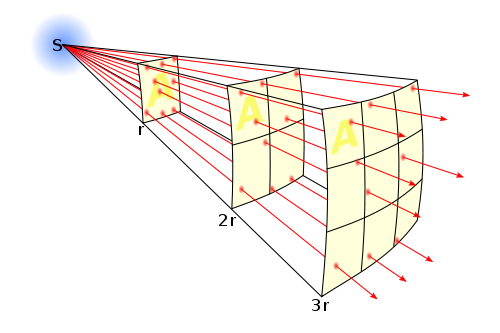
\includegraphics{InverseSquareLaw.png}\hfill}

Through a very simple calculation, it is as simple as
\begin{gather}
\begin{split}L_0 = \frac{ L }{ 4\pi r^2 } .\end{split}\notag\\\begin{split}\end{split}\notag
\end{gather}
We are dealing with Cosmology now. The space-time manifold should be a great concern. The luminosity turns out to be
\begin{gather}
\begin{split}L_0 = \frac{L_\mathrm{abs} }{4\pi d^2} \frac{1}{1+z} \frac{1}{1+z} .\end{split}\notag\\\begin{split}\end{split}\notag
\end{gather}
Here d is the physical distance between the star and the observer. L is the absolute luminosity of the star, which stands for the power of the star. z is the redshift of the star.

The first $\frac{1}{1+z}$ term comes from the fact that the energy of each photon decrease due to expansion of the universe, while the second is the result that the rate of photons arrived at the observer is less.

We are happy to define
\begin{gather}
\begin{split}d_L = d (1+z) ,\end{split}\notag\\\begin{split}\end{split}\notag
\end{gather}
then the luminosity becomes simpler,
\begin{gather}
\begin{split}L_0 = \frac{L_{\mathrm {abs}}}{4\pi d_L^2} .\end{split}\notag\\\begin{split}\end{split}\notag
\end{gather}
Now we come back to have a look at this luminosity.
\begin{itemize}
\item {} 
We can measure how much energy is passing through a unit area at a unit time, which means \textbf{we can determine this luminosity directly from observations}.

\item {} 
We can \textbf{predict the absolute luminosity} from a star evolution model.

\item {} 
The $d_L = d (1+z)$ is only valid for a flat universe, with curvature term $K=0$ in Friedmann equation.

\end{itemize}

Then we can find out this so called luminosity distance
\begin{gather}
\begin{split}d_L = \frac{  L_{\mathrm {abs}} }{ 4\pi L_0 }\end{split}\notag\\\begin{split}\end{split}\notag
\end{gather}
from some data.


\subparagraph{Luminosity Distance from Theory}
\label{Cosmology/cosmoIndex:luminosity-distance-from-theory}
We don't just do the observation for the luminosity distance itself.
We observe to test theories.

What is this distance in theory?
\begin{gather}
\begin{split}d_L = d (1+z)\end{split}\notag\\\begin{split}\end{split}\notag
\end{gather}
Wait, didn't we just mention that this is only valid for a flat universe? So we just do some extension.
\begin{gather}
\begin{split}d_L = R(d) (1+z)\end{split}\notag\\\begin{split}\end{split}\notag
\end{gather}
where R(d) is a function of d and can be determined through geometry,
\begin{itemize}
\item {} 
Spherical: $4\pi \sin^2 d$ ,

\item {} 
Flat: $4\pi d$ ,

\item {} 
Hyperbolic: $4\pi \sinh^2 d$ .

\end{itemize}


\subparagraph{Nearby Objects}
\label{Cosmology/cosmoIndex:nearby-objects}
For nearby objects, we can always use flat geometry and use Taylor expansion at current time for a(t).

Luminosity distance is
\begin{gather}
\begin{split}d_L = d (1+z) = r a(t) (1+z) ,\end{split}\notag\\\begin{split}\end{split}\notag
\end{gather}
where r is the comoving distance and a(t) is the scale factor at time t.

We know
\begin{gather}
\begin{split}r = \int_t^{t_0} \frac{1}{a(t')} \mathrm d t' .\end{split}\notag\\\begin{split}\end{split}\notag
\end{gather}
So we are happy to use Taylor expansion around $t_0$ for $a(t)$, and keep only up to the second order of time. And do some substitution with
\begin{gather}
\begin{split}H_0 = \dot a(t_0)/a(t_0)\end{split}\notag\\\begin{split}q_0=\ddot a (t_0) / a(t_0)\end{split}\notag
\end{gather}
We then do the same thing on redshift
\begin{gather}
\begin{split}z=a(t_0)/a(t) - 1 .\end{split}\notag\\\begin{split}\end{split}\notag
\end{gather}
Finally, we can find out the relation $r(z)$, which leads us to the result we need, $d_L(z) = H_0^{-1} (z - \frac12 (1+q_0) z^2)$.
\begin{itemize}
\item {} 
For very near objects (not as near as our sun of course),
\begin{gather}
\begin{split}d_L = H_0^{-1}z .\end{split}\notag\\\begin{split}\end{split}\notag
\end{gather}
\end{itemize}

\textbf{This is a model independent observation and derivation. We can draw a line to represent the case when deceleration parameter is zero, lines higher than this stands for a accelerating universe while lower region show a decelerating universe.}

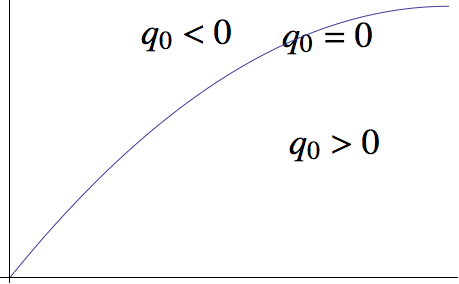
\includegraphics{LuminosityDistanceVSRedshift.png}

We can show that for a vacuum energy dominated universe, the line would go up and for a matter dominated universe, it would below the zero deceleration line.


\subparagraph{Comment}
\label{Cosmology/cosmoIndex:comment}
In this model independent method, the only two parameters occur are Hubble constant $H_0$ and deceleration parameter $q_0$ .


\paragraph{Angular Diameter Distance}
\label{Cosmology/cosmoIndex:angular-diameter-distance}

\subparagraph{Observation}
\label{Cosmology/cosmoIndex:observation}
Angular diameter distance is really useful if we have some standard ruler. Now assume we have a ruler d, we can find out the angle between the two ends of the ruler, by some kind of measurement.

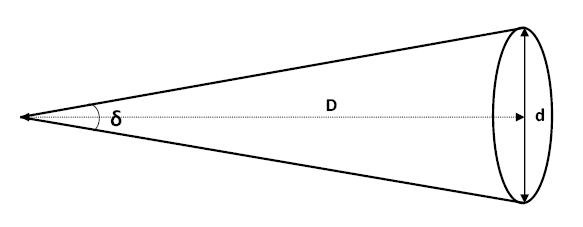
\includegraphics{AngularDiaFormula.jpg}

At the same time, we can use magic of math
\begin{gather}
\begin{split}\theta = d/D .\end{split}\notag\\\begin{split}\end{split}\notag
\end{gather}
Now as we already find out what $\theta$ is by a measurement, and we said about the d is a standard ruler, which means we know the length of it very well. Then we can find out the distance $D$, which is the distance between us and the standard ruler.


\subparagraph{Theory}
\label{Cosmology/cosmoIndex:theory}
We can find out this kind of distance, which we will denote it as $d_A$ from now on. What is it for?

A angular diameter distance is the physical distance between us and the standard ruler,
\begin{gather}
\begin{split}d_A = a(t)r .\end{split}\notag\\\begin{split}\end{split}\notag
\end{gather}
We can use the same trick we used in luminosity distance calculations, and it is easy to find that
\begin{gather}
\begin{split}d_A = H_0^{-1} (z - \frac{1}{2} (3 + q_0)z^2 ) .\end{split}\notag\\\begin{split}\end{split}\notag
\end{gather}
Again, the observation is related to only two parameters, Hubble constant $H_0$ and deceleration parameter $q_0$.


\subparagraph{Standard Rulers}
\label{Cosmology/cosmoIndex:standard-rulers}
It is hard to imagine that we really have some standard rulers. In fact, we do. They are
\begin{itemize}
\item {} 
\href{https://en.wikipedia.org/wiki/Baryon\_acoustic\_oscillations}{Baryon Acoustic Oscillation}

\item {} 
Sound Horizon at Recombination

\end{itemize}


\paragraph{Galaxy Number Count}
\label{Cosmology/cosmoIndex:galaxy-number-count}
Now we can see anything that is only (simply) related to physical or comoving distance can be determined by this trick. The result is that only two cosmological parameters would come in our equation as long as we keep only upper to order two of redshift.

Here another example is the galaxy number count.
\begin{gather}
\begin{split}\frac{\mathrm d N_g}{\mathrm d z \mathrm d\Omega} = z^2 \frac{n_0}{H_0^3}  (1-2(1+q_0) z) .\end{split}\notag\\\begin{split}\end{split}\notag
\end{gather}

\section{Quantum Optics}
\label{Quantum/QuantumOptics:quantum-optics}\label{Quantum/QuantumOptics::doc}

\subsection{Quantum Optics Framework}
\label{Quantum/QuantumOptics:quantum-optics-framework}
From Professor \href{http://info.phys.unm.edu/~ideutsch/Classes/Phys566F13/index.htm\#syllabus}{Ivan Deutsch}.
\begin{enumerate}
\item {} 
Classical foundations
\begin{enumerate}
\item {} 
Oscillators, interference, and coherence.

\item {} 
Simple harmonic oscillators, quadratures, and Fourier analysis.

\item {} 
Lorentz oscillator model.

\end{enumerate}

\item {} 
Quantum foundations
\begin{enumerate}
\item {} 
Density matrix and coherence.

\item {} 
Two level systems -- Pauli algebra, Bloch-sphere, magnetic resonance.

\item {} 
Quantum simple harmonic oscillator.

\end{enumerate}

\item {} 
Optical resonance for two level atoms
\begin{enumerate}
\item {} 
Atom-photon interaction in electric dipole approximation.

\item {} 
Pseudo-spin formulation, Rabi flopping.

\item {} 
Density matrix formulation.

\item {} 
Phenomenological damping -- master equation and rate equations.

\end{enumerate}

\item {} 
The electromagnetic vacuum
\begin{enumerate}
\item {} 
Quantization of the electromagnetic field.

\item {} 
Spontaneous emission and Wigner-Weisskopf theory.

\item {} 
Resonance fluorescence -- Mollow triplet.

\item {} 
Jaynes-Cummings model -- Dressed states.

\end{enumerate}

\item {} 
Three level quantum coherence
\begin{enumerate}
\item {} 
Raman resonance.

\item {} 
Dark states and EIT.

\item {} 
Slow light, fast light, and polaratons.

\end{enumerate}

\item {} 
Quantum-Optical Coherence
\begin{enumerate}
\item {} 
Photon counting statistics -- Mandel's formula.

\item {} 
Theory of partial coherence - Classical statistical optics

\item {} 
Coherent states as quasi-classical states.

\item {} 
Glauber's correlation functions.

\item {} 
Hanbury-Brown and Twiss interferometry.

\item {} 
Bunching, antibunching ,and photon statistics.

\end{enumerate}

\item {} 
Nonclassical Light
\begin{enumerate}
\item {} 
Phase space methods -- Quasiprobability distributions, P-Glauber, Q-Husimi, W-Wigner functions.

\item {} 
Nonlinear optics and nonclassical light.

\item {} 
Squeezed states.

\item {} 
Homodyne detection.

\item {} 
Correlated twin photons.

\item {} 
Photon interferometry.

\end{enumerate}

\end{enumerate}


\chapter{Indices and tables}
\label{index:indices-and-tables}\begin{itemize}
\item {} 
\emph{genindex}

\item {} 
\emph{modindex}

\item {} 
\emph{search}

\end{itemize}


\chapter{License}
\label{index:license}
This work is licensed under a \href{http://creativecommons.org/licenses/by-nc-sa/3.0/}{Attribution-NonCommercial-ShareAlike 3.0}.

{\hfill\scalebox{0.050000}{
\includegraphics{CCBYNCSA.png}}\hfill}



\renewcommand{\indexname}{Index}
\printindex
\end{document}
